% ==========================================
% LatexRefinement Step Output: step4-2026-09-22-tuesday-week2-algebra-1-offset-final.tex
% Model: gemini-3.6-flash
% Temperature: 0.35
% TopP: 0.9
% TopK: 10
% MaxOutputTokens: 65535
% ThinkingBudget: 4096
% ThinkingLevel: HIGH
% Prompt Tokens: 70’067
% Candidates Tokens: 37’364 (inkl. Thinking Tokens)
% Cached Tokens: 0
% Processed on: 2026-10-03 21:06:35
% ==========================================

% Primary Language: English
% End of the video: 01:30:33

\lecturechapter[2]{Tuesday}{22 Sep}{22 September 2026}{Groups, Rings, Ideals, Subrings, and Introduction to Categories}

\begin{overview}[Course Content Overview]
This lecture reviews the fundamental algebraic structures introduced in Week 1---groups, rings, and fields---and explores their intrinsic properties, including the uniqueness of neutral elements and inverses. We formalize structure-preserving mappings (\newterm{group and ring homomorphisms/isomorphisms}), examine classical isomorphism classes over $\mathbb{R}$, and investigate substructures: \newterm{subgroups}, \newterm{ideals}, and \newterm{subrings} (including the classification of subrings and ideals of $\mathbb{Z}$, and ideals in smooth function spaces). Finally, we introduce the foundational language of \newterm{category theory}, defining categories, objects, morphisms, categorical isomorphisms, and \newterm{functors} with concrete algebraic examples.
\end{overview}

\section{Organizational Remarks}

\begin{speech}[00:00:00 - 00:01:48]
Okay, so we start, and there has been some progress on the website. There should be instructions there. Also, first of all, you should be able to register for the problem sessions now. 

The second thing is that there should be instructions on the website about how to upload your homework. 

And the third thing is about the quiz, and I think there's a link there, too. We'll see if it works on Friday. So, the rule for the quiz will be that you can take it anytime from $6$ in the morning on Friday to midnight. And if this is not enough freedom, we can also discuss it. It's not so...

So, another course hack is that if you look at this Metaphor page \inlinemetanote{writes \qt{Metaphor 2018} on the blackboard} in $2018$ --- it was the last time I taught this course ---, that Metaphor page is there. This course is going to follow roughly the same path. In fact, the topics and homework --- I mean, there's maybe some slight switching order of lectures ---, but you can find all the information there. In particular, all the problem sets that Lieke will eventually upload, you can already look at them now if you want to get ahead. 

And also, they're all the answers to all the problem sets. You can also look at them if you want, but in the modern world it's easy to find answers to these questions, so I don't see there's any reason to hide them from you. So, you can find everything there.

So, the other thing is that if you want to ask me a question, I'm happy to talk about math with anybody. You have to find me. Normally, I have an office, but I was kicked out because of this \qt{Fenstersanierung}. And it's going to last forever. So, I have a secret office on this floor. If you find me, you can talk to me. You just have to find it. It's actually pretty hard to find. But if you do, you can knock on the door. Sometimes I'm busy, sometimes I'm not, but I'm happy to talk to anyone. But you have to find the office yourself.
\end{speech}

\begin{note}[Organizational Information: Course Website and Metaphor Archive]
The lecturer outlines administrative details for the semester:
\begin{itemize}
    \item \textbf{Problem Sessions \& Homework:} Registration for exercise sessions is open on the course website, where instructions for online homework submission are posted.
    \item \textbf{Weekly Quizzes:} Friday quizzes can be completed asynchronously between 06:00 and 24:00 (midnight).
    \item \textbf{Course Archive (Metaphor 2018):} Lecture topics, problem sets, and solution sets from the 2018 iteration of the course are publicly accessible for advance study.
    \item \textbf{Office Hours:} Due to ongoing building renovations (\qt{Fenstersanierung}), the lecturer occupies a temporary office on the floor.
\end{itemize}
\end{note}

\section{Review of Groups, Rings, and Fields}

\subsection{Group Axioms and Uniqueness of Identities}

\begin{speech}[00:01:48 - 00:03:22]
Okay, so last week we discussed kind of carefully these three objects which are the centerpiece for this course. 

$G$ is a group \inlinemetanote{writes $(G, \cdot, e)$ on the blackboard}, and last week I used the star ($\star$) for the product. No one does that. That was purely for didactic purposes, and probably pointless didactic purposes. The standard for a group is dot ($\cdot$), but as I said, you can name this anything you want. 

So, this is the standard data of the group, and the group --- I don't repeat everything, but has the three axioms: associativity, existence of the neutral element, and existence of inverses.

So, now this is written now in slightly more abstract language than the explicit equations. And there's many things I didn't say, because they are all, in some sense, part of the definition. Like I didn't say explicitly... you could ask yourself: this neutral element, could there be some other element that also has the neutrality property? So, these are things you should think about yourself. I can't teach you everything; it's not possible. 

Could there be another $\hat{e} \in G$ that has the neutrality property? And the answer is no, because then you could look at $e \cdot \hat{e}$. If I use the fact that $e$ is the neutral element, this equals $\hat{e}$, and if $\hat{e}$ is a pretend neutral element, then this equals $e$. Okay? Is that clear?
\end{speech}

\begin{content}[Definition of a Group and Uniqueness of the Identity]
\begin{definition}[Group]\label[definition]{def:group}
A \newterm{group} is a triple $(G, \cdot, e)$, consisting of a non-empty set $G$, a binary operation $\cdot \colon G \times G \to G$, and a distinguished element $e \in G$ (called the \newterm{identity} or \newterm{neutral element}), satisfying the following three group axioms:
\begin{enumerate}[label=\textbf{(\arabic*)}]
    \item \textbf{Associativity:} For all $a, b, c \in G$,
    \[
    (a \cdot b) \cdot c = a \cdot (b \cdot c).
    \]
    \item \textbf{Existence of a Neutral Element:} There exists an element $e \in G$ such that for all $a \in G$,
    \[
    a \cdot e = e \cdot a = a.
    \]
    \item \textbf{Existence of Inverses:} For every $a \in G$, there exists an element $b \in G$ such that
    \[
    a \cdot b = b \cdot a = e.
    \]
\end{enumerate}
\end{definition}

\begin{proposition}[Uniqueness of the Neutral Element]\label[proposition]{prop:uniqueness-neutral-element}
Let $(G, \cdot)$ be a group. The neutral element $e \in G$ is unique.
\end{proposition}

\begin{proof}
Suppose $e, \hat{e} \in G$ are both neutral elements in $G$. Consider the product $e \cdot \hat{e}$:
\begin{itemize}
    \item Since $e$ is a neutral element, $e \cdot \hat{e} = \hat{e}$.
    \item Since $\hat{e}$ is a neutral element, $e \cdot \hat{e} = e$.
\end{itemize}
Equating both expressions yields:
\[
\hat{e} = e \cdot \hat{e} = e.
\]
Thus, the neutral element is unique.
\end{proof}
\end{content}

\subsection{Uniqueness of Inverses}

\begin{speech}[00:03:22 - 00:05:04]
And then other questions you could have: if $x$ is an element of the group, then this existence of inverse says that there exists a $y$ such that $x \cdot y$ equals the neutral element. And you could say: could there be another $\hat{y}$ where $x \cdot \hat{y}$ is equal to $e$? 

And the answer is no, again. No! And how do you prove this? Well, you look at this equation, and you multiply both sides by the actual --- the first one:
\[
y \cdot (x \cdot \hat{y}) = y \cdot e = y.
\]
And then this thing is equal by the original property --- so the neutral element property is both sides ---, so this thing is equal to $e$, so this is equal to $\hat{y}$. Okay?

Is that clear? So, all of this is embedded in some sense in the definitions. You could define a group by saying that there exists a neutral element and it's unique, there exist inverses and they're unique. You don't have to; you could do that. That's making the definition bigger. 

You can also try to make the definition smaller. There's some kind of strange direction where people think that, well, there's three axioms. We'd like a group to only have two axioms. And some guy in the '60s found some crazy way to write it with just one axiom, but it's just logically equivalent. You can go look that up if you want. I don't remember; it's some complicated axioms, you can imagine.
\end{speech}

\begin{content}[Uniqueness of Inverses in a Group]
\begin{proposition}[Uniqueness of Inverses]\label[proposition]{prop:uniqueness-inverse}
Let $(G, \cdot, e)$ be a group. For each element $x \in G$, the inverse element $y \in G$ satisfying $x \cdot y = y \cdot x = e$ is unique.
\end{proposition}

\begin{proof}
Let $x \in G$. Suppose $y, \hat{y} \in G$ are both inverses of $x$, so that $x \cdot y = y \cdot x = e$ and $x \cdot \hat{y} = \hat{y} \cdot x = e$.

Multiplying the equation $x \cdot \hat{y} = e$ on the left by $y$ gives:
\[
y \cdot (x \cdot \hat{y}) = y \cdot e = y.
\]
Using the associativity of the group operation on the left-hand side:
\[
(y \cdot x) \cdot \hat{y} = y.
\]
Since $y$ is an inverse of $x$, we have $y \cdot x = e$. Substituting this in:
\[
e \cdot \hat{y} = y \implies \hat{y} = y.
\]
Therefore, the inverse of $x$ is unique. We denote this unique inverse by $x^{-1}$.
\end{proof}

\begin{steps}[Why Redundant Axioms Are Omitted]
The standard definition of a group requires only the \emph{existence} of an identity and of inverses. As demonstrated above, their \emph{uniqueness} is not an independent axiom but an immediate logical consequence of associativity and the existence axioms.
\end{steps}
\end{content}

\subsection{Rings and Fields}

\begin{speech}[00:05:04 - 00:06:55]
Okay, so that's the group, and the other structure we had was this ring, which I don't repeat everything again. But the way to think about this is that if I look at just the additive part, this is an abelian group, and then I have some axioms for multiplication, and then two times the distributive laws. So, those were the axioms for the ring, and we did some examples.

So, certainly one part of this class is really internalizing these axioms. And there's some kind of idea about mathematics which is some kind of asymptotic understanding. Which is not just that you understand it, but like the really asymptotic understanding that you try to hope for, which you never really achieve, is that not only do you understand it, but you cannot imagine the state of not understanding it. That's the thing you should really aim for. And you know, you can only do that kind of asymptotically. You can never really achieve that, but with these... So, this is just at the axiomatic level.
\end{speech}

\begin{speech}[00:06:55 - 00:08:02]
And then there was a notion of a field, and the field is somehow... the group is by itself an algebraic object. The field is a particular case of a ring, meaning a field is a ring with some additional structure, and the additional structure is that non-zero elements have multiplicative inverses. 

So, you can think about this: in the whole world of rings, some of them are fields. But rings and groups are separate, although they are related by the fact that the additive part of the ring is an abelian group.

Okay, so those were the structures, and in algebra, after you have structures, there's the notion of the maps that respect the structures, which are the homomorphisms. And you've seen this before, and we discussed a little bit last week, but I want to put them on equal footing here.
\end{speech}

\begin{content}[Review of Rings and Fields]
\begin{definition}[Ring]\label[definition]{def:ring}
A \newterm{ring} is a $5$-tuple $(R, +, \cdot, 0, 1)$ consisting of a set $R$, two binary operations $+$ (addition) and $\cdot$ (multiplication), and two distinguished elements $0, 1 \in R$ ($0 \neq 1$) such that:
\begin{enumerate}[label=\textbf{(\arabic*)}]
    \item $(R, +, 0)$ is an \newterm{abelian group} (i.e., addition is associative, commutative, has identity $0$, and every element has an additive inverse $-a$).
    \item Multiplication $\cdot$ is associative with identity $1$:
    \[
    (a \cdot b) \cdot c = a \cdot (b \cdot c) \quad \text{and} \quad a \cdot 1 = 1 \cdot a = a \quad \forall a, b, c \in R.
    \]
    \item Multiplication distributes over addition from both the left and the right:
    \begin{align*}
    a \cdot (b + c) &= (a \cdot b) + (a \cdot c), \\
    (a + b) \cdot c &= (a \cdot c) + (b \cdot c) \quad \forall a, b, c \in R.
    \end{align*}
\end{enumerate}
\end{definition}

\begin{definition}[Field]\label[definition]{def:field}
A \newterm{field} is a commutative ring $(F, +, \cdot, 0, 1)$ in which every non-zero element possesses a multiplicative inverse:
\[
\forall x \in F \setminus \{0\}, \ \exists x^{-1} \in F \text{ such that } x \cdot x^{-1} = 1.
\]
Equivalently, $(F \setminus \{0\}, \cdot, 1)$ is an abelian group under multiplication.
\end{definition}
\end{content}

\begin{insight}[The Hierarchy of Algebraic Structures]
Algebra organizes mathematical systems by layering structural axioms:
\begin{itemize}
    \item \textbf{Groups $(G, \cdot, e)$:} A single operation with associativity, identity, and inverses.
    \item \textbf{Rings $(R, +, \cdot, 0, 1)$:} Two operations where $(R, +, 0)$ is an abelian group, multiplication is associative with $1$, and the operations are tied together via the distributive laws.
    \item \textbf{Fields $(F, +, \cdot, 0, 1)$:} Commutative rings where $(F \setminus \{0\}, \cdot, 1)$ is also an abelian group.
\end{itemize}
\end{insight}

\begin{aiNote}[Standing Convention: Commutativity of Rings]
As established in Week 1 (\cref{rem:ring-convention}), unless explicitly stated otherwise, the term \textbf{ring} in this course always refers to a \textbf{commutative ring with unity} ($a \cdot b = b \cdot a$ for all $a, b \in R$). Non-commutative rings (such as matrix algebras $M_n(K)$ or endomorphism rings) are treated as specialized exceptions.
\end{aiNote}

\section{Group Homomorphisms and Isomorphisms}

\subsection{Definition and Properties of Homomorphisms}

\begin{speech}[00:08:02 - 00:09:40]
So, if you have two groups, then we want to consider maps that respect the group structure. So, this is called $f$ is a group homomorphism if:
\[
f(a \cdot b) = f(a) \cdot f(b) \quad \text{for all } a, b \in G.
\]

Okay, so last week I did something complicated where we have $G$ is $(G, \star)$ and then $\hat{G}$ is $(\hat{G}, \hat{\star})$ to be completely clear about the products being different. I'm never going to do that again. No one ever does that.

So, here when you read this, this multiplication is the operation in the first one, and that's the operation in the second one. Is that clear? They're both just called dot ($\cdot$). And in fact, many people just don't write it at all. It'd be kind of normal to look in a book and there'd just be nothing, because that's the standard way you deal with algebra. You don't write $x \cdot y$, you just write $xy$.

Okay, so that's the definition of a group homomorphism. It respects the structure. It says you can multiply here and then go over by $f$, or you can go over separately and multiply. That's what's respecting the structure.
\end{speech}

\begin{speech}[00:09:40 - 00:10:40]
Then you could say: what about the neutral element? Why am I not saying anything about the neutral element? I could. I could add $f(e) = \hat{e}$, or if I want to be clear, $\hat{e}$, the $e$ on that side. 

I could add that, but I don't have to, because if I put $e$ here, if I just use this property, I put $f(e \cdot e)$ --- there's only one thing you can do always --- so I just stick $e$ in here. You agree?

And then I use the neutral property on this side: we get $f(e) = f(e) \cdot f(e)$.

And then I can use the cancellation property of the group: $f(e)$ has some inverse. There exists some $y \in \hat{G}$ such that $y \cdot f(e) = \hat{e}$, right? This is the cancellation property. We've used it many times, and at some point I will stop explaining it. 

So, we multiply by $y$ on both sides: we get $y \cdot f(e) = y \cdot (f(e) \cdot f(e))$. So, then this is $\hat{e} = (y \cdot f(e)) \cdot f(e) = \hat{e} \cdot f(e) = f(e)$. So, $f(e) = \hat{e}$. Okay?

So, I don't have to, but you could put it in there.
\end{speech}

\begin{content}[Group Homomorphisms and Preservation of Identities]
\begin{definition}[Group Homomorphism]\label[definition]{def:group-homomorphism}
Let $(G, \cdot, e)$ and $(\hat{G}, \cdot, \hat{e})$ be groups. A function $f \colon G \to \hat{G}$ is called a \newterm{group homomorphism} (or simply \newterm{homomorphism}) if it respects the group operation, that is:
\begin{equation}\label{eq:group-homomorphism}
f(a \cdot b) = f(a) \cdot f(b) \quad \forall a, b \in G.
\end{equation}
\end{definition}

\begin{proposition}[Preservation of the Neutral Element]\label[proposition]{prop:homomorphism-neutral-element}
Let $f \colon G \to \hat{G}$ be a group homomorphism. Then $f$ automatically maps the identity of $G$ to the identity of $\hat{G}$:
\begin{equation}\label{eq:hom-preserves-identity}
f(e) = \hat{e}.
\end{equation}
\end{proposition}

\begin{proof}
Since $e \cdot e = e$ in $G$, applying the homomorphism property yields:
\[
f(e) = f(e \cdot e) = f(e) \cdot f(e).
\]
Since $f(e) \in \hat{G}$ belongs to a group, it possesses an inverse $y \in \hat{G}$ such that $y \cdot f(e) = \hat{e}$. Multiplying both sides of the equation on the left by $y$:
\begin{align}
y \cdot f(e) &= y \cdot \bigl(f(e) \cdot f(e)\bigr) \nonumber \\
\hat{e} &= \bigl(y \cdot f(e)\bigr) \cdot f(e) && \text{(by Associativity)} \nonumber \\
\hat{e} &= \hat{e} \cdot f(e) \nonumber \\
\hat{e} &= f(e). \label{eq:f-e-equals-ehat}
\end{align}
Thus, $f(e) = \hat{e}$.
\end{proof}
\end{content}

\subsection{Group Isomorphisms}

\begin{speech}[00:10:40 - 00:11:47]
So, that's for the group. The group is the algebraic structure, and if you have two groups, you compare them with a homomorphism. It's a map that respects the structure.

And this is following the pattern of this kind of analysis in linear algebra also. There you have two vector spaces, and the map is a linear transformation. That's the notion of the map that respects the vector space structure on both sides.

And then there's some standard things to say: we say $f$ is a group isomorphism if $f$ is a group homomorphism and $f$ is bijective. Okay? So, this should not surprise you. You've seen these terms in linear algebra, right?

Which language did you learn linear algebra in?
\end{speech}

\begin{student}[Student Answer]
English.
\end{student}

\begin{speech}[00:11:49 - 00:13:00]
English, okay, well, that's no problem then.

And there's another way to say this: $f$ is a group isomorphism if and only if there exists an inverse, there exists a group homomorphism in the other direction. There exists a group homomorphism $g \colon \hat{G} \to G$ such that if I do $f$ first and then $g$, I get the identity on the first group, and if I do $g$ first and then $f$, I get the identity on the second group. These are equivalent. Okay?

So, if you have the bottom, it's certainly bijective, because you have the forward and backwards map. And if you have the top, since it's bijective there exists an inverse function, and you have to show that that's a homomorphism, which I leave to you to show. Okay? So, I hope this is clear.
\end{speech}

\begin{content}[Definition and Characterization of Group Isomorphisms]
\begin{definition}[Group Isomorphism]\label[definition]{def:group-isomorphism}
Let $G$ and $\hat{G}$ be groups. A map $f \colon G \to \hat{G}$ is a \newterm{group isomorphism} if:
\begin{enumerate}[label=\textbf{(\arabic*)}]
    \item $f$ is a group homomorphism, and
    \item $f$ is bijective.
\end{enumerate}
If such an isomorphism exists, we say that $G$ and $\hat{G}$ are \newterm{isomorphic} and write $G \cong \hat{G}$.
\end{definition}

\begin{proposition}[Alternative Invertibility Characterization]\label[proposition]{prop:isomorphism-inverse-characterization}
A map $f \colon G \to \hat{G}$ is a group isomorphism if and only if there exists a group homomorphism $g \colon \hat{G} \to G$ such that:
\begin{equation}\label{eq:isomorphism-inverses}
g \circ f = \operatorname{id}_G \quad \text{and} \quad f \circ g = \operatorname{id}_{\hat{G}}.
\end{equation}
\end{proposition}

\begin{proof}
\textbf{Direction ($\Leftarrow$):} If such a homomorphism $g$ exists, the two-sided inverse equations $g \circ f = \operatorname{id}_G$ and $f \circ g = \operatorname{id}_{\hat{G}}$ imply by standard set theory that $f$ is a bijection. Since $f$ is also given as a homomorphism, $f$ is an isomorphism.

\textbf{Direction ($\Rightarrow$):} If $f$ is an isomorphism, it is a bijective homomorphism, so a set-theoretic inverse function $g = f^{-1} \colon \hat{G} \to G$ exists satisfying \eqref{eq:isomorphism-inverses}. It remains only to verify that $g$ is a homomorphism. For any $\hat{a}, \hat{b} \in \hat{G}$, let $a = g(\hat{a})$ and $b = g(\hat{b})$, so that $f(a) = \hat{a}$ and $f(b) = \hat{b}$. Then:
\[
f(a \cdot b) = f(a) \cdot f(b) = \hat{a} \cdot \hat{b}.
\]
Applying $g = f^{-1}$ to both sides gives:
\[
g(\hat{a} \cdot \hat{b}) = a \cdot b = g(\hat{a}) \cdot g(\hat{b}).
\]
Thus, $g$ is a group homomorphism.
\end{proof}
\end{content}

\section{Examples of Groups and Isomorphisms over \texorpdfstring{$\mathbb{R}$}{R}}

\subsection{Three Classical Groups of Real Numbers}

\begin{speech}[00:13:00 - 00:15:26]
All right, so maybe an example. 

If I take the real numbers, one group is the real numbers with addition and zero: $(\mathbb{R}, +, 0)$. This is a rather basic group: real numbers, zero, you can add them.

Another group which you maybe don't think about as much is you could take the non-zero real numbers, multiplication, and one: $(\mathbb{R}^*, \cdot, 1)$. So, here I just remind you --- this is pretty standard ---, when you have a field and you put a star ($^*$), this usually means you take the field and you throw out the zero:
\[
\mathbb{R}^* := \mathbb{R} \setminus \{0\}.
\]
Is that clear? So, this is the non-zero real numbers, and I put multiplication, one. That is also a group. Are you happy with that? Because you can invert non-zero elements.

And there's another one here: there's kind of two ways to be non-zero: you can be positive, or you can be negative. So, I could take the positive ones: $(\mathbb{R}_{>0}^*, \cdot, 1)$. That's still a group. Is that clear?

If I try to then take the negative ones, I kind of get in trouble because if I multiply negative ones I get positive, and the one is not there. So, anyway, there's these three groups.

So, which of these are isomorphic? Or which ones are not isomorphic? Do you know this? Let me write the question: Which are isomorphic? Which means: for which ones can I find an isomorphism?
\end{speech}

\begin{content}[Three Standard Groups over $\mathbb{R}$]
We consider the following three algebraic groups defined on subsets of $\mathbb{R}$:
\begin{enumerate}[label=\textbf{(\arabic*)}]
    \item \textbf{The Additive Group of Real Numbers:}
    \[
    (\mathbb{R}, +, 0)
    \]
    where $+$ is standard addition, $0$ is the neutral element, and the inverse of $x$ is $-x$.
    \item \textbf{The Multiplicative Group of Non-Zero Real Numbers:}
    \[
    (\mathbb{R}^*, \cdot, 1) \quad \text{where } \mathbb{R}^* := \mathbb{R} \setminus \{0\},
    \]
    equipped with standard multiplication, identity $1$, and inverse $x^{-1} = \frac{1}{x}$.
    \item \textbf{The Multiplicative Group of Positive Real Numbers:}
    \[
    (\mathbb{R}_{>0}^*, \cdot, 1) \quad \text{where } \mathbb{R}_{>0}^* := \{x \in \mathbb{R} \mid x > 0\},
    \]
    which forms a group under multiplication since the product and inverse of positive numbers remain strictly positive.
\end{enumerate}
\end{content}

\subsection{Non-Isomorphism between \texorpdfstring{$(\mathbb{R}^*, \cdot, 1)$}{(R*, *, 1)} and \texorpdfstring{$(\mathbb{R}_{>0}^*, \cdot, 1)$}{(R>0*, *, 1)}}

\begin{speech}[00:15:26 - 00:16:21]
So, let's start with these --- this is maybe the more confusing one. If I take the non-zero real numbers, multiplication, $1$, and I take the positive ones, $(\mathbb{R}_{>0}^*, \cdot, 1)$, could these be isomorphic?

It's kind of strange, because if you draw the picture, one of them is kind of both sides, and the other one is just one side. So, it seems kind of unlikely, although, you know, there's still bijections that do this. There are set-theoretic bijections, because both sets are just uncountable sets; they have the same cardinality.

What do you think?

Yeah?
\end{speech}

\begin{student}[Student Answer]
No, because we run into a problem for $-1$, because if we had if $f(-1)$...
\end{student}

\begin{speech}[00:16:30 - 00:16:33]
Which way is $f$ going?
\end{speech}

\begin{student}[Student Answer continued]
So, $f$ goes from $\mathbb{R}^*$ to $\mathbb{R}_{>0}^*$.
\end{student}

\begin{speech}[00:16:37 - 00:16:39]
Yeah.
\end{speech}

\begin{student}[Student Answer continued]
And then $f(1)$ has to be $1$.
\end{student}

\begin{speech}[00:16:42 - 00:16:45]
Has to be $1$, that's the...
\end{speech}

\begin{student}[Student Answer continued]
Yeah, that's $1$, but that's also $f(-1)$ squared.
\end{student}

\begin{speech}[00:16:48 - 00:16:50]
Yeah, so $f(-1)$ equals what? That's a good...
\end{speech}

\begin{student}[Student Answer continued]
$f(-1) \cdot f(-1)$ will be $1$, so the only positive number such that times itself is $1$ will be $1$, so $f(-1)$ has to be $1$. So, $f(1) = f(-1)$, and then it's not bijective.
\end{student}

\begin{speech}[00:17:09 - 00:18:00]
Yeah, this is all correct. So, the simplest way to say it is that $f(-1)$ has to be a square root of $1$, okay, by this law. And there's only one square root of $1$ in the positive, and that's already taken by $1$. So, it violates the bijectivity.

Do you understand this statement? The point is that $1$ has two square roots in here. There are two elements when you multiply them by themselves you get $1$: $+1$ and $-1$. And those two elements have to go to two different elements here, because it's a bijection. If there were a bijection, they would have to go to two different elements. But here there's only one element whose square is $1$. So, it's impossible that there is a bijection. Okay? 

So, this is a solid argument. This is the standard argument.
\end{speech}

\begin{content}[Non-Isomorphism of \texorpdfstring{$(\mathbb{R}^*, \cdot, 1)$}{(R*, *, 1)} and \texorpdfstring{$(\mathbb{R}_{>0}^*, \cdot, 1)$}{(R>0*, *, 1)}]
\begin{proposition}\label[proposition]{prop:rstar-not-isom-rpos}
The groups $(\mathbb{R}^*, \cdot, 1)$ and $(\mathbb{R}_{>0}^*, \cdot, 1)$ are not isomorphic:
\[
(\mathbb{R}^*, \cdot, 1) \not\cong (\mathbb{R}_{>0}^*, \cdot, 1).
\]
\end{proposition}

\begin{proof}
Suppose for contradiction that there exists an isomorphism $f \colon \mathbb{R}^* \to \mathbb{R}_{>0}^*$.

By \cref{prop:homomorphism-neutral-element}, any homomorphism must preserve the identity:
\begin{equation}\label{eq:f-of-one}
f(1) = 1.
\end{equation}
Now consider the element $-1 \in \mathbb{R}^*$. Since $(-1) \cdot (-1) = 1$, the homomorphism property implies:
\[
f(-1)^2 = f(-1) \cdot f(-1) = f\bigl((-1) \cdot (-1)\bigr) = f(1) = 1.
\]
Thus, $f(-1)$ must be a real root of the equation $t^2 = 1$ in the codomain $\mathbb{R}_{>0}^*$.
In the set of positive real numbers $\mathbb{R}_{>0}^*$, the only solution to $t^2 = 1$ is $t = 1$. Therefore:
\begin{equation}\label{eq:f-of-minus-one}
f(-1) = 1.
\end{equation}
Comparing \eqref{eq:f-of-one} and \eqref{eq:f-of-minus-one}, we obtain $f(1) = f(-1) = 1$. Since $1 \neq -1$ in $\mathbb{R}^*$, this contradicts the injectivity of $f$. Consequently, no such isomorphism can exist.
\end{proof}

\begin{steps}[Algebraic Invariants: Torsion Elements]
This proof illustrates the power of \newterm{algebraic invariants}: an algebraic property preserved by all isomorphisms. In $(\mathbb{R}^*, \cdot, 1)$, the element $-1$ is an element of order $2$ (an element $x \neq e$ such that $x^2 = e$, called a \newterm{torsion element}). However, $(\mathbb{R}_{>0}^*, \cdot, 1)$ contains no elements of order $2$. Since an isomorphism must map elements of order $k$ to elements of order $k$, the two groups cannot be isomorphic despite having the same uncountable cardinality ($2^{\aleph_0}$) as sets.
\end{steps}
\end{content}

\subsection{Isomorphism between \texorpdfstring{$(\mathbb{R}, +, 0)$}{(R, +, 0)} and \texorpdfstring{$(\mathbb{R}_{>0}^*, \cdot, 1)$}{(R>0*, *, 1)}}

\begin{speech}[00:18:00 - 00:18:22]
And what about this one? $(\mathbb{R}, +, 0)$ and $(\mathbb{R}_{>0}^*, \cdot, 1)$?

If I make any mistakes on the board, you have to tell me, all right?

So, what about this? Could these be isomorphic?

Yeah?
\end{speech}

\begin{student}[Student Answer]
I think it could, we can take $f$ from $\mathbb{R}$ to $\mathbb{R}_{>0}^*$ by the function $e$ to the power of $x$.
\end{student}

\begin{speech}[00:18:32 - 00:19:30]
Yeah, yeah. This is like the most famous function in mathematics, and this is its purpose, actually. 

This is by $\exp$, $\exp(x)$, so $f(x) = \exp(x)$. So, you take a number, and you get a positive number. If you take $0$, you get $1$. And the main property of $\exp$ is that it intertwines the addition here with the multiplication there.

So, this is actually the most famous function in mathematics, basically, and this is its role. It gives you an isomorphism, a group isomorphism, between the additive structure and the multiplicative structure.

So, that's a kind of weird thing. It's saying that actually from the point of view of the group, the group doesn't see the difference between the additive structure and the multiplicative structure of the reals.
\end{speech}

\begin{content}[The Exponential Isomorphism]
\begin{proposition}\label[proposition]{prop:r-additive-isom-rpos-mult}
The additive group of real numbers $(\mathbb{R}, +, 0)$ is isomorphic to the multiplicative group of positive real numbers $(\mathbb{R}_{>0}^*, \cdot, 1)$:
\[
(\mathbb{R}, +, 0) \cong (\mathbb{R}_{>0}^*, \cdot, 1).
\]
\end{proposition}

\begin{proof}
Define the map $f \colon \mathbb{R} \to \mathbb{R}_{>0}^*$ by the exponential function:
\begin{equation}\label{eq:exp-map}
f(x) := \exp(x) = e^x.
\end{equation}
We verify the two isomorphism conditions:
\begin{enumerate}[label=\textbf{(\arabic*)}]
    \item \textbf{Homomorphism Property:} For all $x, y \in \mathbb{R}$, by the functional equation of the exponential function:
    \[
    f(x + y) = e^{x+y} = e^x \cdot e^y = f(x) \cdot f(y).
    \]
    Thus, $f$ transforms addition in $(\mathbb{R}, +)$ into multiplication in $(\mathbb{R}_{>0}^*, \cdot)$.
    \item \textbf{Bijectivity:} The exponential function $\exp \colon \mathbb{R} \to \mathbb{R}_{>0}^*$ is strictly monotonically increasing and continuous, with an explicit two-sided inverse given by the natural logarithm:
    \[
    g \colon \mathbb{R}_{>0}^* \to \mathbb{R}, \quad g(y) := \ln(y).
    \]
    For all $x \in \mathbb{R}$, $g(f(x)) = \ln(e^x) = x = \operatorname{id}_{\mathbb{R}}(x)$, and for all $y \in \mathbb{R}_{>0}^*$, $f(g(y)) = e^{\ln(y)} = y = \operatorname{id}_{\mathbb{R}_{>0}^*}(y)$.
\end{enumerate}
Therefore, $f$ is a group isomorphism.
\end{proof}
\end{content}

\begin{insight}[The Fundamental Role of the Exponential Function]
From an algebraic perspective, the exponential function $x \mapsto e^x$ is not merely an analytic power series or a solution to $y' = y$; its primary algebraic purpose is to establish an exact equivalence (\newterm{group isomorphism}) between the continuous additive world $(\mathbb{R}, +)$ and the continuous positive multiplicative world $(\mathbb{R}_{>0}^*, \cdot)$.
\end{insight}

\section{The Kernel and Subgroups}

\subsection{Definition and Properties of the Kernel}

\begin{speech}[00:19:30 - 00:21:10]
There's a notion of a subgroup. We did this for the ring; I'm going to repeat it all for the ring in one second. So, if you have this map, $f \colon G \to \hat{G}$ --- and I'm not going to keep saying group homomorphism. The standard is to say homomorphism, which is abbreviated $\operatorname{hom}$, and you're supposed to understand, since I'm talking about groups, it's a group homomorphism.

All right, so if $f$ is a group homomorphism, then from the spirit of linear algebra, which is the algebra you're supposed to be most familiar with, if you have a linear transformation between two vector spaces, the thing you immediately study is the kernel and the image of that linear transformation. So, we can do that also with groups.

So, then we can consider the kernel and the image, but let's start with the kernel. So, what properties does this kernel enjoy?

The kernel of a group homomorphism is defined to be those elements in $G$ such that when I apply $f$, I get the neutral element on the second side. In the linear algebra language, it's things that went to zero, so now it's the elements that go to the neutral element. Is that clear?

Well, the neutral element itself is in here. That's one property, because the homomorphism takes the neutral element here to the neutral element there. So, that's there, right?
\end{speech}

\begin{speech}[00:21:10 - 00:22:15]
Second property: suppose $a$ and $b$ are in the kernel of $f$, then what can we say? We can consider what happens to $f(ab)$. 

There's only one thing we can do here. These proofs at this level are strong proofs, meaning that there's only one thing you can do at every stage, and you just have to do it. 

So, this is $f(a) \cdot f(b)$, and now the assumption is they're both in the kernel, so these are both $\hat{e} \cdot \hat{e}$, and then we use the identity property, so that's $\hat{e}$. 

Okay, so what have we learned here? That says that if $a$ and $b$ are in the kernel, we have proven that $a \cdot b$ is in the kernel. Okay?
\end{speech}

\begin{content}[Definition and Closure Properties of the Kernel]
\begin{definition}[Kernel of a Group Homomorphism]\label[definition]{def:kernel}
Let $f \colon G \to \hat{G}$ be a group homomorphism between groups $(G, \cdot, e)$ and $(\hat{G}, \cdot, \hat{e})$. The \newterm{kernel} of $f$, denoted $\ker(f)$, is the pre-image of the identity element $\hat{e} \in \hat{G}$:
\begin{equation}\label{eq:kernel-def}
\ker(f) := \bigl\{ x \in G \;\big|\; f(x) = \hat{e} \bigr\} \subseteq G.
\end{equation}
\end{definition}

\begin{proposition}[Properties of the Kernel: Identity and Product Closure]\label[proposition]{prop:kernel-properties-part1}
Let $f \colon G \to \hat{G}$ be a group homomorphism. Then $\ker(f)$ satisfies:
\begin{enumerate}[label=\textbf{(\arabic*)}]
    \item \textbf{Contains the Identity:} $e \in \ker(f)$.
    \item \textbf{Closed under the Group Product:} If $a, b \in \ker(f)$, then $a \cdot b \in \ker(f)$.
\end{enumerate}
\end{proposition}

\begin{proof}
\textbf{Property (1):} By \cref{prop:homomorphism-neutral-element}, $f(e) = \hat{e}$. Thus, $e \in \ker(f)$ by definition.

\textbf{Property (2):} Let $a, b \in \ker(f)$, which means $f(a) = \hat{e}$ and $f(b) = \hat{e}$. Using the homomorphism property of $f$:
\[
f(a \cdot b) = f(a) \cdot f(b) = \hat{e} \cdot \hat{e} = \hat{e}.
\]
Therefore, $a \cdot b \in \ker(f)$.
\end{proof}
\end{content}

\subsection{Closure under Inverses and the Definition of Subgroups}

\begin{speech}[00:22:15 - 00:24:05]
So, we're looking at properties of the kernel, and we have discovered that the neutral element's in the kernel, and the kernel is closed under the group law, the product.

We might be curious now whether the inverses are there also.

So, that's the third property of the kernel: if $x$ is in the kernel of $f$, then the inverse... 

I should make this comment that very often the inverse for the group law is denoted $x^{-1}$. That's just the name of it. The axioms say there exists an inverse. This is very often the name that's given to it. This kind of presupposes that the product you're calling dot ($\cdot$). If the product you're calling is plus ($+$), then you usually use the minus sign ($-x$) here. But this is just notation. You could call it anything you want. You could call it Fred, or an elephant, anything. We're calling it this, okay?

Then that's the inverse is also in the kernel. Okay?
\end{speech}

\begin{speech}[00:24:05 - 00:26:00]
And how are you going to prove this? You have to start out by taking $f(x \cdot x^{-1})$. That's the one thing you know. 

On the one hand, this is $f(e)$, and that's $\hat{e}$. On the other hand, this is $f(x) \cdot f(x^{-1})$, and this thing is assumed to be in the kernel, so this is equal to $\hat{e} \cdot f(x^{-1})$.

So, we get that the neutral element is equal to neutral element times that ($\hat{e} = \hat{e} \cdot f(x^{-1})$), so that must be the neutral element. Okay? We could go one more if we want to be really explicit:
\[
f(x^{-1}) = \hat{e} \cdot f(x^{-1}) = \hat{e}.
\]
So, now we have the full chain: $f(x^{-1}) = \hat{e}$.

So, we have these three properties: that the kernel enjoys these three properties. It contains the neutral element of $G$, the source group, it's closed under the group product, and it's closed under inverses.

Definition: if $H$ is a subset of $G$, then $H$ is a subgroup if $e \in H$, $H$ is closed under the product, and $H$ is closed under inverses. Meaning if anybody's in $H$, then its multiplicative inverse is also in $H$, okay?
\end{speech}

\begin{content}[Closure of the Kernel under Inverses and the Subgroup Axioms]
\begin{proposition}[Closure of the Kernel under Inverses]\label[proposition]{prop:kernel-closure-inverses}
Let $f \colon G \to \hat{G}$ be a group homomorphism. If $x \in \ker(f)$, then $x^{-1} \in \ker(f)$.
\end{proposition}

\begin{proof}
Let $x \in \ker(f)$, so that $f(x) = \hat{e}$. Consider the image of the identity element $e = x \cdot x^{-1}$:
\begin{align*}
\hat{e} &= f(e) && \text{(by \cref{prop:homomorphism-neutral-element})} \\
&= f(x \cdot x^{-1}) \\
&= f(x) \cdot f(x^{-1}) && \text{(homomorphism property)} \\
&= \hat{e} \cdot f(x^{-1}) && \text{(since } x \in \ker(f)\text{)} \\
&= f(x^{-1}) && \text{(neutral element property in } \hat{G}\text{)}.
\end{align*}
Thus, $f(x^{-1}) = \hat{e}$, which demonstrates that $x^{-1} \in \ker(f)$.
\end{proof}

\begin{definition}[Subgroup]\label[definition]{def:subgroup}
Let $(G, \cdot, e)$ be a group, and let $H \subseteq G$ be a non-empty subset. $H$ is called a \newterm{subgroup} of $G$ (denoted $H \le G$) if it satisfies the following three conditions:
\begin{enumerate}[label=\textbf{(\arabic*)}]
    \item \textbf{Identity Element:} $e \in H$.
    \item \textbf{Closure under Multiplication:} For all $a, b \in H$, $a \cdot b \in H$.
    \item \textbf{Closure under Inverses:} For all $x \in H$, $x^{-1} \in H$.
\end{enumerate}
\end{definition}

\begin{steps}[Inherited Group Structure]
If $H \subseteq G$ satisfies these three axioms, the restriction of the group operation $\cdot|_{H \times H}$ defines a binary operation on $H$, associativity is inherited from $G$, and $e \in H$ acts as the identity with inverses in $H$. Consequently, $(H, \cdot, e)$ is itself a group in its own right.
\end{steps}
\end{content}

\subsection{The Kernel and the Image as Subgroups}

\begin{speech}[00:26:00 - 00:26:50]
So, in particular, this implies that if I take $H$ and I take the group law, which makes sense on $H$ because $H$ is closed under it, and I take the zero, which also makes sense because zero's in $H$, that this is a group.

Which is a very nice thing. A subgroup is a group. It'd be terrible if it weren't, right?

So, that's the definition for a subgroup. And now we've proven a little proposition: The kernel of $f$ is a subgroup of $G$.

Is that clear?
\end{speech}

\begin{content}[Subgroup Property of the Kernel]
\begin{proposition}[Kernel as a Subgroup]\label[proposition]{prop:kernel-is-subgroup}
Let $f \colon G \to \hat{G}$ be a group homomorphism. Then the kernel $\ker(f)$ is a subgroup of the domain group $G$:
\begin{equation}\label{eq:kernel-subgroup}
\ker(f) \le G.
\end{equation}
\end{proposition}

\begin{proof}
By \cref{prop:homomorphism-neutral-element}, $e \in \ker(f)$. By \cref{prop:kernel-properties-part1}, $\ker(f)$ is closed under multiplication. By \cref{prop:kernel-closure-inverses}, $\ker(f)$ is closed under taking inverses. Hence, by \cref{def:subgroup}, $\ker(f) \le G$.
\end{proof}
\end{content}

\subsection{The Image of a Group Homomorphism}

\begin{speech}[00:26:50 - 00:28:30]
Okay, so that's the investigation of the kernel and the notion of a subgroup. But there's also the image. And so proposition --- and I leave this for you, you can prove it ---: The image of $f$ is a subgroup of $\hat{G}$.

So, how do you prove this? You just check that the image contains the neutral element... it has to because the neutral element from the first group goes to the neutral element of the second group, so the image has to contain the neutral element. And then you have to check that if we have two elements in the image, then if I apply the group law for $\hat{G}$, they stay in the image, and the inverse. The proofs are all just the same. You just follow your nose. There's only one thing you can do, and you can do it.

All right. So, this is a nice situation for groups, that the understanding of the group is by these very simple axioms. There's lots of examples; in fact, part of this class is the examples for the groups, which will come later. And whenever you have a homomorphism, there's the kernel and the image.

So, this one I leave to you. You can look in the books too, but it's not worth looking in the books. You should read the books, I take it back. But the problem with reading such a simple thing in the book is that you have to learn what notation the author is using and all that. It's much simpler just to write the proof of this yourself.
\end{speech}

\begin{content}[The Image of a Group Homomorphism]
\begin{definition}[Image of a Homomorphism]\label[definition]{def:group-image}
Let $f \colon G \to \hat{G}$ be a group homomorphism. The \newterm{image} of $f$, denoted $\operatorname{Im}(f)$ (or $f(G)$), is the set:
\begin{equation}\label{eq:image-def}
\operatorname{Im}(f) := \bigl\{ \hat{y} \in \hat{G} \;\big|\; \exists x \in G \text{ such that } f(x) = \hat{y} \bigr\} \subseteq \hat{G}.
\end{equation}
\end{definition}

\begin{proposition}[Image as a Subgroup]\label[proposition]{prop:image-is-subgroup}
Let $f \colon G \to \hat{G}$ be a group homomorphism. Then the image $\operatorname{Im}(f)$ is a subgroup of the codomain group $\hat{G}$:
\begin{equation}\label{eq:image-subgroup}
\operatorname{Im}(f) \le \hat{G}.
\end{equation}
\end{proposition}

\begin{proof}
We verify the three subgroup conditions for $\operatorname{Im}(f) \subseteq \hat{G}$:
\begin{enumerate}[label=\textbf{(\arabic*)}]
    \item \textbf{Identity Element:} Since $f(e) = \hat{e}$ by \cref{prop:homomorphism-neutral-element}, $\hat{e} \in \operatorname{Im}(f)$.
    \item \textbf{Closure under Multiplication:} Let $\hat{y}_1, \hat{y}_2 \in \operatorname{Im}(f)$. Then there exist $x_1, x_2 \in G$ such that $f(x_1) = \hat{y}_1$ and $f(x_2) = \hat{y}_2$. Using the homomorphism property:
    \[
    \hat{y}_1 \cdot \hat{y}_2 = f(x_1) \cdot f(x_2) = f(x_1 \cdot x_2).
    \]
    Since $x_1 \cdot x_2 \in G$, we have $\hat{y}_1 \cdot \hat{y}_2 \in \operatorname{Im}(f)$.
    \item \textbf{Closure under Inverses:} Let $\hat{y} \in \operatorname{Im}(f)$ with $\hat{y} = f(x)$ for some $x \in G$. Since $x^{-1} \in G$, we compute:
    \[
    \hat{y} \cdot f(x^{-1}) = f(x) \cdot f(x^{-1}) = f(x \cdot x^{-1}) = f(e) = \hat{e}.
    \]
    By uniqueness of inverses in $\hat{G}$, $\hat{y}^{-1} = f(x^{-1}) \in \operatorname{Im}(f)$.
\end{enumerate}
Thus, $\operatorname{Im}(f) \le \hat{G}$.
\end{proof}
\end{content}

\begin{speech}[00:28:30 - 00:29:39]
But actually, I'm a big fan of books. It's one way to understand this kind of classical history of mathematics: read a lot of math books. And I know that somehow in the modern world, this is less popular, but in my generation we read a lot of math books.

And on the topic of books, there's the book for the course, which was picked a while ago, not by me even, and it has the advantage that it's freely available on the ETH website, so you can just click it and... Then there's some other references I gave which are, I think, a little bit better books. They're more advanced in perspective, they're written better.

But I think they're not freely available on the webpage, so it wasn't chosen for this class. But it's a good idea to read books. You'll learn something.
\end{speech}

\begin{note}[Pedagogical Aside: Recommended Literature]
The lecturer emphasizes the pedagogical value of reading classical mathematical texts and consulting textbook references, noting the freely available course textbook on the ETH website alongside advanced supplementary reading.
\end{note}

\section{Ring Homomorphisms, Ideals, and Subrings}

\subsection{Ring Homomorphisms and Isomorphisms}

\begin{speech}[00:29:39 - 00:31:49]
Okay, so for the ring, we had also defined what a homomorphism is: it's a ring homomorphism. If I have two rings, then we had defined $f$ is a ring hom, which, as I said, I will just say hom and you're supposed to understand they're rings. And then the axioms for a ring hom, if you remember, the first one is:
\[
f(a+b) = f(a) + f(b).
\]
And the interpretation of this: it says that the additive part of this is a group and the additive part of that is a group, and the ring hom should be a group hom for those parts. Is that clear? So, additively $f$ is a group hom for the plus part, okay?

Of course, we also have this, which respects the multiplication: $f(ab) = f(a)f(b)$.

And then we also have that the identity has to be respected: $f(1) = 1$.

Okay? So, those are the notions of the ring homomorphism. And again, a ring isomorphism is a bijective ring homomorphism.

And another way to think about it is if there's an isomorphism, then that means that the inverse is a ring homomorphism in the other direction, just as I said with groups.
\end{speech}

\begin{content}[Review of Ring Homomorphisms and Isomorphisms]
\begin{definition}[Ring Homomorphism]\label[definition]{def:ring-homomorphism}
Let $(R, +, \cdot, 0, 1)$ and $(\hat{R}, +, \cdot, \hat{0}, \hat{1})$ be rings. A map $f \colon R \to \hat{R}$ is a \newterm{ring homomorphism} if for all $a, b \in R$:
\begin{enumerate}[label=\textbf{(\arabic*)}]
    \item \textbf{Additive Homomorphism:} $f(a + b) = f(a) + f(b)$ (i.e., $f \colon (R, +, 0) \to (\hat{R}, +, \hat{0})$ is a group homomorphism on the additive group).
    \item \textbf{Multiplicative Homomorphism:} $f(a \cdot b) = f(a) \cdot f(b)$.
    \item \textbf{Preservation of the Multiplicative Identity:} $f(1) = \hat{1}$.
\end{enumerate}
\end{definition}

\begin{definition}[Ring Isomorphism]\label[definition]{def:ring-isomorphism}
A ring homomorphism $f \colon R \to \hat{R}$ is called a \newterm{ring isomorphism} if $f$ is bijective. Equivalently, $f$ is an isomorphism if and only if there exists a ring homomorphism $g \colon \hat{R} \to R$ such that $g \circ f = \operatorname{id}_R$ and $f \circ g = \operatorname{id}_{\hat{R}}$.
\end{definition}
\end{content}

\subsection{The Kernel of a Ring Homomorphism and Ideals}

\begin{speech}[00:31:49 - 00:34:03]
Okay, so then we can do the parallel study: if $f \colon R \to \hat{R}$ is a ring homomorphism, there are two things I can study as before: the kernel of $f$ and the image of $f$. And we had studied the kernel last week: for the group, both the kernel and image were subgroups: the former was the subgroup of the source group and the latter was the subgroup of the target group. But for rings, the symmetry is broken, so one has to concentrate a bit here.

And that's also true for vector spaces. For vector spaces, you have a linear map, the kernel is the subspace of the first one, and the image is the subspace of the second one. For the ring, something different happens.

And for the kernel of $f$, we had proven last week that the kernel of $f$ is something called an ideal. An ideal $I$ of a ring satisfies the following condition: one condition on the additive structure is that $(I, +, 0)$ inside $(R, +, 0)$ is a subgroup. That's the additive structure.
\end{speech}

\begin{speech}[00:34:03 - 00:35:23]
So for an ideal, there's kind of two pieces. One is how it works additively, and it must be a subgroup, and it's not a surprise because we already said that $f$ on the additive structures is a group homomorphism, and we already know that the kernel from the point of view of the group homomorphism is an additive subgroup.

And then the second has to do with the multiplicative part. The kernel satisfies this property that if I take any element of the ring $r \in R$ and any element of the ideal $x \in I$, then $r \cdot x$ is in the ideal. So, these are the two conditions that define an ideal. And the proposition last week was: the kernel is an ideal. All right?

So, what about the image? Is the image an ideal? What is the image? The answer is no. Ideal is the notion for the kernel. The image is something else: the image is a subring.
\end{speech}

\begin{content}[Ideals in Rings and the Kernel as an Ideal]
\begin{definition}[Ideal]\label[definition]{def:ideal}
Let $(R, +, \cdot, 0, 1)$ be a commutative ring. A subset $I \subseteq R$ is called an \newterm{ideal} (denoted $I \trianglelefteq R$) if it satisfies:
\begin{enumerate}[label=\textbf{(\arabic*)}]
    \item \textbf{Additive Subgroup:} $(I, +, 0)$ is a subgroup of $(R, +, 0)$, i.e.,
    \[
    0 \in I, \quad \forall x, y \in I \implies x + y \in I, \quad \text{and} \quad \forall x \in I \implies -x \in I.
    \]
    \item \textbf{Multiplicative Absorption (Ideal Property):} For every element of the ring $r \in R$ and every element of the ideal $x \in I$, the product belongs to $I$:
    \[
    \forall r \in R, \ \forall x \in I \implies r \cdot x \in I.
    \]
\end{enumerate}
\end{definition}

\begin{aiNote}[Ideals and Commutativity]
Because $R$ is assumed commutative, left ideals ($r \cdot x \in I$), right ideals ($x \cdot r \in I$), and two-sided ideals ($r \cdot x \cdot s \in I$) coincide. In non-commutative ring theory, these concepts diverge, and kernels of ring homomorphisms are always two-sided ideals.
\end{aiNote}

\begin{proposition}[The Kernel of a Ring Homomorphism is an Ideal]\label[proposition]{prop:kernel-ring-hom-ideal}
Let $f \colon R \to \hat{R}$ be a ring homomorphism. Then the kernel $\ker(f) := \{x \in R \mid f(x) = \hat{0}\}$ is an ideal of $R$.
\end{proposition}

\begin{proof}
We verify the two ideal conditions for $\ker(f)$:
\begin{enumerate}[label=\textbf{(\arabic*)}]
    \item \textbf{Additive Subgroup:} Since $f \colon (R, +, 0) \to (\hat{R}, +, \hat{0})$ is a group homomorphism between abelian groups, $\ker(f)$ is an additive subgroup of $(R, +, 0)$ by \cref{prop:kernel-is-subgroup}.
    \item \textbf{Multiplicative Absorption:} Let $r \in R$ and $x \in \ker(f)$, so $f(x) = \hat{0}$. Using the multiplicative homomorphism property:
    \[
    f(r \cdot x) = f(r) \cdot f(x) = f(r) \cdot \hat{0} = \hat{0}.
    \]
    Thus, $r \cdot x \in \ker(f)$.
\end{enumerate}
Therefore, $\ker(f) \trianglelefteq R$.
\end{proof}
\end{content}

\begin{insight}[Broken Symmetry: Subrings vs. Ideals]
In group theory and linear algebra, substructures are uniform: the kernel and image of a homomorphism are both subgroups (or vector subspaces). In ring theory, this symmetry is broken:
\begin{itemize}
    \item The \textbf{kernel} $\ker(f)$ is an \textbf{ideal} (it absorbs multiplication from the entire ring, but does not contain $1$ unless $\hat{R} = \{0\}$).
    \item The \textbf{image} $\operatorname{Im}(f)$ is a \textbf{subring} (it contains the identity $1$, but does not absorb multiplication from outside the image).
\end{itemize}
\end{insight}

\subsection{Subrings and the Image of a Ring Homomorphism}

\begin{speech}[00:36:04 - 00:37:50]
So, what is a subring? Let $R$ be a ring. Whenever I say let $R$ be a ring, you should be thinking that I have in mind all the data: $(R, +, \cdot, 0, 1)$.

A subring $S$ of $R$ satisfies the following properties --- this is the definition. The first property is that $0$ and $1$ should be in the subring. The second is that $S$ is closed under the two operations: whenever I have elements of the subring, I can either add them or multiply them, and they stay in the subring, okay? And the third is that $(S, +, \cdot, 0, 1)$ is a ring. A subring inside here has $0$ and $1$, it's closed under the operations, and together it's a ring. This means it has the additive inverses and things like that, okay?
\end{speech}

\begin{speech}[00:37:50 - 00:40:21]
And so the proposition here is: if I have a ring homomorphism, then the image of $f$ in the second one is a subring.

The kernel is an ideal, the image is a subring. You have to check that the image satisfies these properties. Does the image have $0$? The answer is yes, because on the additive structure, it's a homomorphism of groups, and $0$ goes to $0$. Does the image have $1$? Well, that's part of the definition of a ring homomorphism, so it has $1$. Then you have to check whether it's closed under $+$ and $\cdot$, and you just check that by writing out the equations. And whether this is a ring, you have to check whether it has the additive inverses, but that's also clear.

Okay. So, it's good to have these ideas extremely clear in your head: you have the group, you have the ring, there's a notion of group hom, there's a notion of ring hom, and there's kernel and image in both cases. For the group, the kernel and the image are subgroups; for the ring, something different happens: the image is a subring, but the kernel is an ideal. And so now we should do some examples.
\end{speech}

\begin{content}[Definition of a Subring and the Image of a Ring Homomorphism]
\begin{definition}[Subring]\label[definition]{def:subring}
Let $(R, +, \cdot, 0, 1)$ be a commutative ring with unity. A subset $S \subseteq R$ is called a \newterm{subring} of $R$ (denoted $S \le R$) if:
\begin{enumerate}[label=\textbf{(\roman*)}]
    \item \textbf{Contains Neutral Elements:} $0 \in S$ and $1 \in S$.
    \item \textbf{Closure under Addition and Multiplication:} For all $a, b \in S$,
    \[
    a + b \in S \quad \text{and} \quad a \cdot b \in S.
    \]
    \item \textbf{Ring Axioms (Closure under Additive Inverses):} $(S, +, \cdot, 0, 1)$ is itself a commutative ring with the induced operations (in particular, $-a \in S$ for all $a \in S$).
\end{enumerate}
\end{definition}

\begin{proposition}[The Image of a Ring Homomorphism is a Subring]\label[proposition]{prop:image-ring-hom-subring}
Let $f \colon R \to \hat{R}$ be a ring homomorphism. Then the image $\operatorname{Im}(f) \subseteq \hat{R}$ is a subring of $\hat{R}$.
\end{proposition}

\begin{proof}
We check the subring conditions for $\operatorname{Im}(f)$:
\begin{enumerate}[label=\textbf{(\arabic*)}]
    \item \textbf{Neutral Elements:} Since $f \colon (R, +, 0) \to (\hat{R}, +, \hat{0})$ is a group homomorphism, $f(0) = \hat{0} \in \operatorname{Im}(f)$. By axiom \textbf{(3)} of ring homomorphisms, $f(1) = \hat{1} \in \operatorname{Im}(f)$.
    \item \textbf{Closure under Addition and Multiplication:} Let $\hat{a}, \hat{b} \in \operatorname{Im}(f)$ with $\hat{a} = f(a)$ and $\hat{b} = f(b)$ for $a, b \in R$. Then:
    \[
    \hat{a} + \hat{b} = f(a) + f(b) = f(a + b) \in \operatorname{Im}(f),
    \]
    \[
    \hat{a} \cdot \hat{b} = f(a) \cdot f(b) = f(a \cdot b) \in \operatorname{Im}(f).
    \]
    \item \textbf{Additive Inverses:} For $\hat{a} = f(a) \in \operatorname{Im}(f)$, $-\hat{a} = -f(a) = f(-a) \in \operatorname{Im}(f)$.
\end{enumerate}
Thus, $\operatorname{Im}(f)$ is a subring of $\hat{R}$.
\end{proof}
\end{content}

\section{Examples of Ideals and Subrings}

\subsection{The Even Integers \texorpdfstring{$2\mathbb{Z}$}{2Z} in \texorpdfstring{$\mathbb{Z}$}{Z}}

\begin{speech}[00:40:21 - 00:40:57]
Okay, let's try here: $2\mathbb{Z}$ inside $\mathbb{Z}$. So, this is a ring, $\mathbb{Z}$. I can take the even integers. 

So, what is this inside that? Is it an ideal? Is it a subring? 

What's the answer?
\end{speech}

\begin{student}[Student Answer]
I think it is an ideal.
\end{student}

\begin{speech}[00:41:00 - 00:41:35]
It's an ideal. So, claim: this is an ideal. 

Why is it an ideal? We have to check that additively it's a subgroup: if you add two even numbers you get an even number, $0$ is an even number, if you have an even number the minus of it is an even number, so you're totally solid on the subgroup. Then if you take any other element of the integers and multiply it by an even number, you stay even. So, that looks pretty good. Answer is yes. 

Okay, what about a subring? Is it a subring?
\end{speech}

\begin{student}[Student Answer]
No, because we don't have the $1$.
\end{student}

\begin{speech}[00:41:38 - 00:41:48]
Yeah, so it's not a subring. Ideal: yes. Subring: no. 

Okay, so let's try something else.
\end{speech}

\begin{content}[The Even Integers: Ideal vs. Subring]
\begin{example}[The Even Integers $2\mathbb{Z} \subset \mathbb{Z}$]\label[example]{ex:even-integers-ideal}
Let $R = \mathbb{Z}$ and consider the subset of even integers $2\mathbb{Z} := \{ 2k \mid k \in \mathbb{Z} \}$.
\begin{itemize}
    \item \textbf{$2\mathbb{Z}$ is an Ideal of $\mathbb{Z}$ (\textcolor{ForestGreen}{YES}):}
    \begin{enumerate}[label=\textbf{(\arabic*)}]
        \item $(2\mathbb{Z}, +, 0)$ is an additive subgroup of $\mathbb{Z}$: $0 = 2 \cdot 0 \in 2\mathbb{Z}$, the sum of two even integers $2k + 2\ell = 2(k + \ell)$ is even, and $-(2k) = 2(-k) \in 2\mathbb{Z}$.
        \item Multiplicative absorption holds: For any $r \in \mathbb{Z}$ and any $x = 2k \in 2\mathbb{Z}$,
        \[
        r \cdot x = r \cdot (2k) = 2(r \cdot k) \in 2\mathbb{Z}.
        \]
    \end{enumerate}
    \item \textbf{$2\mathbb{Z}$ is NOT a Subring of $\mathbb{Z}$ (\textcolor{BrickRed}{NO}):}
    The multiplicative identity $1 \notin 2\mathbb{Z}$ since $1$ is odd.
\end{itemize}
\end{example}
\end{content}

\subsection{Subrings between \texorpdfstring{$\mathbb{Z}$}{Z} and \texorpdfstring{$\mathbb{Q}$}{Q}}

\begin{speech}[00:41:48 - 00:42:37]
Okay, this is maybe a trickier question. 

Certainly $\mathbb{Z}$ is a subring of $\mathbb{Q}$. I hope that's not controversial. You accept that $\mathbb{Z}$ is a subring of $\mathbb{Q}$? 

Can you find a subring that's in between $\mathbb{Z}$ and $\mathbb{Q}$? Does there exist a subring in between $\mathbb{Z} \subsetneq S \subsetneq \mathbb{Q}$? 

How about that? Can you do that? You have $3$ minutes.
\end{speech}

\begin{student}[Student Answer]
So we look at pairs of integers and denominator is just powers of two?
\end{student}

\begin{speech}[00:42:44 - 00:44:10]
Okay, that's good. So, he is saying that we let $S$ be the set of rational numbers of this form $\frac{a}{2^n}$, where $a$ is an integer and $n$ is also an integer. Is this exactly what you're saying? 

Okay, so that's a proposal. One thing that's good about this proposal is this set $S$ is certainly more than $\mathbb{Z}$ because it has like $3/2$ in it, and it's certainly less than $\mathbb{Q}$ because it doesn't have $2/3$ in it. So, that part is solid. 

Then the claim is you have to check that this satisfies all these properties. What are the properties about having $0$ and $1$? Basically the answer is yes, it's going to satisfy, because you need to know how to add fractions, which I don't teach you. I've never taught anyone how to add fractions; I'm not going to teach you. But when you think about the rule about adding fractions, you keep the $2^n$ in the bottom, that's the main thing here. When you add fractions, the denominator doesn't give you things that you didn't put in. 

And so the answer is yes. This is true. 

So, that's an example. That's a very important one. Of course, $2$ is not important here; you could have put here $17$, it'd be fine. That's another example. And in fact, being prime is not that important either.
\end{speech}

\begin{content}[Subrings of the Rational Numbers]
\begin{example}[{Dyadic Rationals $\mathbb{Z}[\frac{1}{2}] \subset \mathbb{Q}$}]\label[example]{ex:dyadic-rationals-subring}
Consider the problem of finding an intermediate subring strictly between $\mathbb{Z}$ and $\mathbb{Q}$:
\[
\mathbb{Z} \subsetneq S \subsetneq \mathbb{Q}.
\]
Define the set of \newterm{dyadic rationals} $S = \mathbb{Z}[\frac{1}{2}]$ by:
\begin{equation}\label{eq:dyadic-rationals-def}
S := \left\{ \frac{a}{2^n} \;\middle|\; a \in \mathbb{Z}, \ n \in \mathbb{N}_{\ge 0} \right\} \subset \mathbb{Q}.
\end{equation}
\begin{itemize}
    \item \textbf{Proper Inclusions:} $S \supsetneq \mathbb{Z}$ since $\frac{1}{2} = \frac{1}{2^1} \in S \setminus \mathbb{Z}$, and $S \subsetneq \mathbb{Q}$ since $\frac{1}{3} \notin S$ (powers of $2$ cannot produce a denominator divisible by $3$).
    \item \textbf{Subring Verification:}
    \begin{enumerate}[label=\textbf{(\roman*)}]
        \item $0 = \frac{0}{2^0} \in S$ and $1 = \frac{1}{2^0} \in S$.
        \item Closed under addition: For $\frac{a}{2^n}, \frac{b}{2^m} \in S$ with $n \ge m$,
        \[
        \frac{a}{2^n} + \frac{b}{2^m} = \frac{a + b \cdot 2^{n-m}}{2^n} \in S.
        \]
        \item Closed under multiplication: $\frac{a}{2^n} \cdot \frac{b}{2^m} = \frac{a \cdot b}{2^{n+m}} \in S$.
        \item Closed under additive inverses: $-\left(\frac{a}{2^n}\right) = \frac{-a}{2^n} \in S$.
    \end{enumerate}
\end{itemize}
Thus, $\mathbb{Z}[\frac{1}{2}]$ is a subring of $\mathbb{Q}$. More generally, for any $m \in \mathbb{Z}_{\ge 2}$ (e.g., $m = 17$), the localized ring $\mathbb{Z}[\frac{1}{m}] := \{ \frac{a}{m^n} \mid a \in \mathbb{Z}, n \ge 0 \}$ forms a proper intermediate subring $\mathbb{Z} \subsetneq \mathbb{Z}[\frac{1}{m}] \subsetneq \mathbb{Q}$.
\end{example}
\end{content}

\subsection{Polynomial Subrings: \texorpdfstring{$\mathbb{Z}[x^2] \subset \mathbb{Z}[x]$}{Z[x^2] in Z[x]}}

\begin{speech}[00:44:10 - 00:45:05]
Okay, so another example. 

Do we get a bell? I don't remember. Do I get to go to the bell, or do I have to stop? 

Okay, let's try one more example before the bell, hopefully. 

If I look at polynomials here, these are polynomials in the variable $x$, that's a ring: $\mathbb{Z}[x]$. Inside it are polynomials in the variable $x^2$: $\mathbb{Z}[x^2]$. Every polynomial in the variable $x^2$ is a polynomial in $x$, so this is a subset: $\mathbb{Z}[x^2] \subset \mathbb{Z}[x]$. I hope that's clear. 

So, is this an ideal, or a subring, or both, or neither, or what?

You ran out of time. Okay, we take a break, you can think about it.
\end{speech}

\begin{pause}[Mid-Lecture Break]
The lecturer announces a short pause for the students to consider whether $\mathbb{Z}[x^2] \subset \mathbb{Z}[x]$ is an ideal or a subring. The lecture resumes at timestamp 00:45:06.
\end{pause}

\begin{speech}[00:45:06 - 00:45:48]
Okay, so maybe we start, or is it a minute? 

I don't know whether we get a bell, I don't remember, but anyway. So, what's the answer to this question?

Yeah?
\end{speech}

\begin{student}[Student Answer]
I'd say it's a subring but not an ideal.
\end{student}

\begin{speech}[00:45:48 - 00:46:22]
Yeah, so subring: yes. Ideal: no. So, for the subring, again, you just have to check that everything's there. 

\inlinemetanote{The bell rings}
Oh, we do get a bell. 

So, why is it not an ideal? Yeah?
\end{speech}

\begin{student}[Student Answer]
If you take $x^2$, and multiply by $x$, then you get $x^3$, which is not in the set.
\end{student}

\begin{speech}[00:46:22 - 00:46:37]
So, $x^2$ is in this, and if it were an ideal, then I should be able to take any $r$ in the ring and multiply it by this $x^2$. So, I take any $r$ in the ring, multiply by $x^2$, it should stay in here. That's if it were an ideal. 

So, I could take $r$ to be $x$, and then this would be odd, and it wouldn't be in there, okay? So, you can check it yourself. 

These are not supposed to be hard questions; it's just about whether you have absorbed the definitions. Which, as I said, is not an easy task.
\end{speech}

\begin{content}[Polynomial Subrings with Even Powers]
\begin{example}[{Even Degree Polynomials $\mathbb{Z}[x^2] \subset \mathbb{Z}[x]$}]\label[example]{ex:even-polynomials-subring}
Let $R = \mathbb{Z}[x]$ be the polynomial ring over $\mathbb{Z}$, and consider the subset $\mathbb{Z}[x^2] \subset \mathbb{Z}[x]$ of polynomials containing only even powers of $x$:
\begin{equation}\label{eq:even-polynomials-def}
\mathbb{Z}[x^2] := \left\{ \sum_{k=0}^m a_k (x^2)^k = a_0 + a_1 x^2 + a_2 x^4 + \dots + a_m x^{2m} \;\middle|\; a_k \in \mathbb{Z} \right\}.
\end{equation}
\begin{itemize}
    \item \textbf{$\mathbb{Z}[x^2]$ is a Subring of $\mathbb{Z}[x]$ (\textcolor{ForestGreen}{YES}):}
    $0, 1 \in \mathbb{Z}[x^2]$, the sum and difference of even polynomials are even, and the product of even powers yields even powers ($x^{2k} \cdot x^{2\ell} = x^{2(k+\ell)}$). Thus, $\mathbb{Z}[x^2] \le \mathbb{Z}[x]$.
    \item \textbf{$\mathbb{Z}[x^2]$ is NOT an Ideal of $\mathbb{Z}[x]$ (\textcolor{BrickRed}{NO}):}
    Taking $r = x \in \mathbb{Z}[x]$ and $p(x) = x^2 \in \mathbb{Z}[x^2]$, their product is:
    \[
    r \cdot p(x) = x \cdot x^2 = x^3 \notin \mathbb{Z}[x^2]
    \]
    since $x^3$ has an odd degree. Thus, $\mathbb{Z}[x^2]$ fails the multiplicative absorption property.
\end{itemize}
\end{example}
\end{content}

\subsection{Subrings of the Integers \texorpdfstring{$\mathbb{Z}$}{Z}}

% [TIMESTAMP-SUSPECT: inspect manually — original: 00:46:37 - 00:47:30]
\begin{speech}[00:46:37 - 00:47:30]
Okay, so let's go to the integers. What are the subrings? 

We've seen the rational numbers have lots of interesting subrings, because we found some: there's the integers, and you could invert $2$, invert $3$, $17$. But what are the subrings of $\mathbb{Z}$?

Yeah?
\end{speech}

\begin{student}[Student Answer]
Only $\mathbb{Z}$.
\end{student}

\begin{speech}[00:46:54 - 00:47:30]
Yeah. There's no real interesting subrings: only $\mathbb{Z}$ in $\mathbb{Z}$. That's the only subring. 

The whole ring is always a subring, just by definition. And this is the only one. 

And why is that? Because the subring would have to contain $1$. And once it contains $1$, it contains every positive number. But the subring also is a subgroup, so it has to contain the negative ones too. 

Okay? So, there's nothing you can do.
\end{speech}

\begin{content}[Classification of the Subrings of the Integers]
\begin{proposition}[Subrings of $\mathbb{Z}$]\label[proposition]{prop:subrings-of-z}
The only subring of $(\mathbb{Z}, +, \cdot, 0, 1)$ is $\mathbb{Z}$ itself:
\begin{equation}\label{eq:subrings-of-z}
S \le \mathbb{Z} \implies S = \mathbb{Z}.
\end{equation}
\end{proposition}

\begin{proof}
Let $S \le \mathbb{Z}$ be a subring.
\begin{enumerate}[label=\textbf{(\arabic*)}]
    \item By definition of a subring, $1 \in S$.
    \item Since $S$ is closed under addition, by induction $n = \underbrace{1 + 1 + \dots + 1}_{n \text{ times}} \in S$ for all positive integers $n \in \mathbb{N}_{>0}$.
    \item By definition, $0 \in S$.
    \item Since $(S, +, 0)$ is an additive subgroup, $S$ is closed under additive inverses: $-n \in S$ for all $n \in \mathbb{N}_{>0}$.
\end{enumerate}
Combining these, $S$ contains all integers $\mathbb{Z} \subseteq S$. Since $S \subseteq \mathbb{Z}$ by assumption, $S = \mathbb{Z}$.
\end{proof}

\begin{steps}[Contrast: Ideals vs. Subrings in $\mathbb{Z}$]
This result highlights the sharp contrast between subrings and ideals in the ring of integers $\mathbb{Z}$:
\begin{itemize}
    \item \textbf{Subrings of $\mathbb{Z}$:} There is only \textbf{one} subring, namely $\mathbb{Z}$ itself (because a subring must contain $1$, which generates all of $\mathbb{Z}$ additively).
    \item \textbf{Ideals of $\mathbb{Z}$:} There are \textbf{infinitely many} distinct ideals of $\mathbb{Z}$, each of the form $n\mathbb{Z} = \langle n \rangle$ for $n \in \mathbb{N}_{\ge 0}$ (because an ideal does not need to contain $1$).
\end{itemize}
\end{steps}
\end{content}

\subsection{Classification of Ideals of \texorpdfstring{$\mathbb{Z}$}{Z}}

\begin{speech}[00:47:30 - 00:48:25]
So, what are the ideals? What are the ideals of $\mathbb{Z}$? 

What would you guess the answer to this question is?

Yeah?
\end{speech}

\begin{student}[Student Answer]
The set of multiples of an integer.
\end{student}

\begin{speech}[00:48:25 - 00:49:35]
Yeah, so you pick some integer $n$, and you look at the multiples of $n$. 

That's the standard notation: $n \cdot \mathbb{Z}$. So, if $n$ is $2$, it's the even numbers; if $n$ is $3$, it's the numbers divisible by $3$, and so on. 

Comment 1: this is certainly an ideal. It's just because the way we checked carefully that $2$, the even ones, were an ideal, it's the same argument, okay?

Comment 2: it's not sensitive to whether you put $+n$ or $-n$ here, because inside $\mathbb{Z}$ is a $-1$. So, if you put $+7$ or $-7$, it's the same set. Is that also clear?

So, typically when you write $n\mathbb{Z}$, you should take $n \ge 0$. You don't have to, but that's the convention. In the literature, you'll never see minus... it's just a weird thing to do. There's no reason...
\end{speech}

\begin{content}[Principal Ideals of the Integers $\mathbb{Z}$]
\begin{definition}[Principal Ideals of $\mathbb{Z}$]\label[definition]{def:principal-ideals-z}
For each integer $n \in \mathbb{Z}$, the set of integer multiples of $n$:
\begin{equation}\label{eq:n-z-def}
n\mathbb{Z} := \{ n \cdot k \mid k \in \mathbb{Z} \}
\end{equation}
is an ideal of $\mathbb{Z}$.
\end{definition}

\begin{remark}[Conventions on $n\mathbb{Z}$]\label[remark]{rem:nz-conventions}
\begin{itemize}
    \item \textbf{Ideals of $\mathbb{Z}$:} For every $n \in \mathbb{Z}$, $(n\mathbb{Z}, +, 0)$ is an additive subgroup of $\mathbb{Z}$, and for any $r \in \mathbb{Z}$ and $x = nk \in n\mathbb{Z}$, $r \cdot x = n(rk) \in n\mathbb{Z}$.
    \item \textbf{Sign Invariance:} Since $-1 \in \mathbb{Z}$ is a unit, $(-n)\mathbb{Z} = n\mathbb{Z}$. By convention, we restrict the generator index to $n \in \mathbb{N}_{\ge 0} = \{0, 1, 2, \dots\}$.
\end{itemize}
\end{remark}
\end{content}

\subsection{Historical Origin of Ideals and David Hilbert}

\begin{speech}[00:49:35 - 00:50:40]
So, we're going to prove these are all the ideals. But this is an important example because the word ideal, where does it come from? The idea is that it's an idealized number, idealized integer. 

For the integers, the ideals are the integers, but when you think about other rings, the ideals are some kind of idea of a number. This was in some sense the origin of this word ideal here: ideal number. This terminology goes back to about $1900$, and there were lots of people around, but certainly one person who played a role was the great David Hilbert, who was a mathematician in Göttingen. And a piece of math culture: does anyone know what the epitaph on the grave of David Hilbert is?

Not one person?

Yeah?
\end{speech}

\begin{student}[Student Question]
What is an epitaph?
\end{student}

\begin{speech}[00:50:40 - 00:51:45]
Ah, epitaph! So, you have a gravestone \inlinemetanote{draws a sketch of an arched gravestone on the blackboard}, and then what's written here? There's the person's name, and then there's like a little motto or slogan. That's the epitaph. 

Okay, so this is a real piece of math culture, what's the epitaph of David Hilbert's grave. This is the kind of thing you learn to be a mathematician; it's part of being in the culture. Yeah, do you know it?
\end{speech}

\begin{student}[Student Answer]
Wir müssen wissen, wir werden wissen.
\end{student}

\begin{speech}[00:51:45 - 00:52:30]
Yeah: \qt{Wir müssen wissen, wir werden wissen.} Two lines. It's in Göttingen. 

\inlinemetanote{The lecturer writes \qt{Motto / Slogan} inside the drawn gravestone on the board, and then erases it}

I have to teach you some culture, too, you know. 

Okay, so we have to prove something.
\end{speech}

\begin{content}[Historical Context: Ideal Numbers and David Hilbert]
\begin{center}

\begin{tikzpicture}[scale=1.1]
    % Gravestone body
    \draw[thick, fill=gray!10] (-1.5, 0) -- (-1.5, 2.0) arc (180:0:1.5) -- (1.5, 0) -- cycle;
    \draw[thick] (-1.8, 0) -- (1.8, 0);
    
    % Inscription
    \node[font=\bfseries] at (0, 2.3) {David Hilbert};
    \node[font=\footnotesize, text=gray!70] at (0, 1.9) {1862 -- 1943};
    \draw[thin, gray!50] (-1.0, 1.6) -- (1.0, 1.6);
    \node[font=\itshape\small] at (0, 1.1) {\qt{Wir müssen wissen,}};
    \node[font=\itshape\small] at (0, 0.6) {\qt{wir werden wissen.}};
\end{tikzpicture}
\end{center}

\begin{steps}[Origin of the Term \qt{Ideal}]
The concept of an \newterm{ideal} originated in algebraic number theory with Ernst Kummer (1840s) as \qt{ideal complex numbers} to restore unique prime factorization in rings of algebraic integers such as $\mathbb{Z}[\zeta_p]$, and was later formalized by Richard Dedekind and David Hilbert around 1900. In $\mathbb{Z}$, every ideal is represented by a concrete integer ($I = n\mathbb{Z}$); in more general rings, ideals generalize the behavior of numbers.
\end{steps}
\end{content}

\subsection{Proof: Every Ideal in \texorpdfstring{$\mathbb{Z}$}{Z} is Principal}

\begin{content}
\begin{theorem}[Ideals of $\mathbb{Z}$ are Principal]\label[theorem]{thm:ideals-of-z-are-principal}
Every ideal $I$ of the ring of integers $\mathbb{Z}$ is of the form:
\begin{equation}\label{eq:ideal-is-nz}
I = n\mathbb{Z} = \langle n \rangle
\end{equation}
for a uniquely determined non-negative integer $n \in \mathbb{N}_{\ge 0}$.
\end{theorem}
\end{content}

\begin{proofWrapper}[Proof that Every Ideal in $\mathbb{Z}$ is of the Form $n\mathbb{Z}$]

\begin{speech}[00:52:30 - 00:54:10]
What do we have to prove? 

Let $I \subseteq \mathbb{Z}$ be an ideal. 

I want to prove it's $n\mathbb{Z}$. What about math what I like is truth. Proof is good, but truth is better. And this stuff is true, but anyway, we should prove it; it's a math course. 

So, if you want to prove it: \textbf{Case (1)} is that $I$ could be just the zero set ($\{0\}$). And this means it's $0 \cdot \mathbb{Z}$. It's a degenerate case. That's possible. And that's an ideal: $0$ is an ideal. 

So, \textbf{Case (2)} is that $I$ has some non-zero element.
\end{speech}

\begin{content}[Proof: Case 1 and Identification of Positive Elements]
\textbf{Case 1 ($I = \{0\}$):} \\
If $I = \{0\}$, then $I = 0\mathbb{Z}$ with $n = 0$. This settles the degenerate case.

\textbf{Case 2 ($I \neq \{0\}$):} \\
If $I$ contains a non-zero element $x \in I$ with $x \neq 0$:
\begin{itemize}
    \item If $x > 0$, then $I$ contains a positive integer.
    \item If $x < 0$, since $I$ is an ideal and $-1 \in \mathbb{Z}$, $-x = (-1) \cdot x \in I$, where $-x > 0$.
\end{itemize}
In either case, the set of positive elements $I \cap \mathbb{N}_{>0}$ is non-empty.
\end{content}

\begin{speech}[00:54:10 - 00:55:40]
Because $I$ has to have $0$ because $I$ is an additive subgroup. If you're not in this case, you have to have some non-zero element. 

Let's call that element $x$. $x$ is in $I$. 

Now, $x$ is an integer. 

So, we can multiply by $\pm 1$ and get a positive integer. One of these is a positive integer. 

So, if it has a non-zero element, then $I$ has a positive integer. 

And if it has a positive integer, what am I going to say now? 

Yeah?
\end{speech}

\begin{student}[Student Answer]
It has a minimum.
\end{student}

\begin{speech}[00:55:40 - 00:57:00]
Yeah, has a least positive integer. That's the next line. 

So, $I$ has a least positive integer. 

Basically every property of integers at some point you have to use this principle. So, once it has a least positive integer, let's call that one $n$. So, $n$ is equal to the least positive integer of $I$. 

So, now we have to show that $I$ is actually $n\mathbb{Z}$. That's what we want to show, all right? 

You look at $y \in I$. There's only one thing you can do now, which is the division algorithm. The division algorithm says $y$ is equal to some multiple of $n$ plus a remainder term:
\[
y = q \cdot n + r.
\]
That is the division, long division.
\end{speech}

\begin{content}[Application of the Well-Ordering Principle and Division Algorithm]
\textbf{Selection of the Minimal Generator $n$:} \\
By the \newterm{Well-Ordering Principle} of $\mathbb{N}$, the non-empty subset $I \cap \mathbb{N}_{>0} \subseteq \mathbb{N}$ contains a unique smallest element:
\begin{equation}\label{eq:n-least-positive}
n := \min(I \cap \mathbb{N}_{>0}).
\end{equation}

\textbf{Claim:} $I = n\mathbb{Z}$.
\begin{itemize}
    \item \textbf{Inclusion $n\mathbb{Z} \subseteq I$:} Since $n \in I$ and $I$ is an ideal, for any $k \in \mathbb{Z}$, $k \cdot n \in I$. Thus, $n\mathbb{Z} \subseteq I$.
    \item \textbf{Inclusion $I \subseteq n\mathbb{Z}$:} Let $y \in I$ be an arbitrary element. By the \newterm{Division Algorithm} (division with remainder in $\mathbb{Z}$), there exist unique integers $q, r \in \mathbb{Z}$ such that:
    \begin{equation}\label{eq:division-algorithm}
    y = q \cdot n + r \quad \text{with} \quad 0 \le r < n.
    \end{equation}
\end{itemize}
\end{content}

\begin{speech}[00:57:00 - 00:58:30]
And the important part of this remainder term is $0 \le r < n$. 

Suppose $y$ is not in $n\mathbb{Z}$, that means that it's not divisible, so there is a remainder term. 

But this remainder term is equal to $y - qn$, and so the remainder term is also in $I$, because $y$ is in $I$, $n$ is in $I$ so $qn$ is in $I$, and since $I$ is an additive subgroup, this is also in $I$. 

It can't be zero because otherwise it would divide, so the long division says $r$ is between $0$ and $n$. 

But then $r$ is a lesser positive integer, which is a contradiction. Okay, that's the proof.
\end{speech}

\begin{speech}[00:58:30 - 00:59:10]
So, we use what you have to use for integers: you use this fact that non-empty subsets have a least one. Once you have that least one, you know what you're trying to prove, and then you use the long division algorithm and use the remainder. This is what you always do with these kind of elementary properties of integers. 

So, that proves this claim. 

And that's the most basic properties of the ideals in the integers.
\end{speech}

\begin{content}[Conclusion of the Proof: Minimality Contradiction]
\begin{proof}[Continuation of Proof of \cref{thm:ideals-of-z-are-principal}]
Rearranging equation \eqref{eq:division-algorithm} for the remainder $r$:
\[
r = y - q \cdot n.
\]
Since $y \in I$, $n \in I$, and $I$ is an ideal, $q \cdot n \in I$. Since $(I, +, 0)$ is an additive subgroup:
\[
r = y - q \cdot n \in I.
\]
We now analyze the remainder $r$:
\begin{itemize}
    \item If $r > 0$, then $r \in I \cap \mathbb{N}_{>0}$ with $r < n$. But this directly contradicts the defining minimality of $n = \min(I \cap \mathbb{N}_{>0})$ from \eqref{eq:n-least-positive}.
    \item Therefore, we must have $r = 0$.
\end{itemize}
Setting $r = 0$ in \eqref{eq:division-algorithm} gives $y = q \cdot n \in n\mathbb{Z}$. Since $y \in I$ was arbitrary, $I \subseteq n\mathbb{Z}$.
Combining both inclusions yields $I = n\mathbb{Z}$.
\end{proof}
\end{content}

\end{proofWrapper}

\begin{insight}[Principal Ideal Domains (PIDs)]
A ring in which every ideal is generated by a single element (i.e., $I = \langle a \rangle = aR$) is called a \newterm{Principal Ideal Domain} (\newterm{PID}). \Cref{thm:ideals-of-z-are-principal} proves that the ring of integers $\mathbb{Z}$ is a PID.
\end{insight}

\subsection{Rings of Smooth Functions and Compactly Supported Ideals}

\begin{speech}[00:59:10 - 01:00:50]
For any ring $R$, we've seen before that $\{0\}$ is an ideal, and the whole ring $R$ is an ideal. 

And we haven't discussed fields at all today, but we discussed last time that if you have a field, these are the only two ideals. 

But the integers have a lot of ideals: all these $n\mathbb{Z}$ are ideals. 

Okay, so let's throw in another example. One object you certainly know in mathematics: if I take the real numbers, you can take $C^\infty$ functions. 

You don't have to take $C^\infty$, you could take $17$ times differentiable functions, but we'll just go $\infty$. These are infinitely differentiable functions. 

So an element here is some function $f \colon \mathbb{R} \to \mathbb{R}$, which I can differentiate as many times as I want, so it has a nice graph; I can graph it like this \inlinemetanote{sketches a wavy function curve on the board}. 

And this beautiful object is a ring. 

Because why? You can add functions, you can multiply functions, $0$ is just the constant function $0$, and $1$ is the constant function $1$. 

Is that clear? It's a ring.
\end{speech}

\begin{content}[The Ring of Smooth Functions \texorpdfstring{$C^\infty(\mathbb{R})$}{C^infty(R)}]
\begin{definition}[Ring of Smooth Functions]\label[definition]{def:smooth-functions-ring}
The set of infinitely differentiable functions on the real line:
\begin{equation}\label{eq:c-infty-def}
C^\infty(\mathbb{R}) := \bigl\{ f \colon \mathbb{R} \to \mathbb{R} \;\big|\; f \text{ is smooth} \bigr\}
\end{equation}
forms a commutative ring $(C^\infty(\mathbb{R}), +, \cdot, 0, 1)$ under pointwise operations:
\begin{align*}
(f + g)(x) &:= f(x) + g(x), \\
(f \cdot g)(x) &:= f(x) \cdot g(x),
\end{align*}
with additive identity $0(x) \equiv 0$ and multiplicative identity $1(x) \equiv 1$.
\end{definition}

\begin{center}
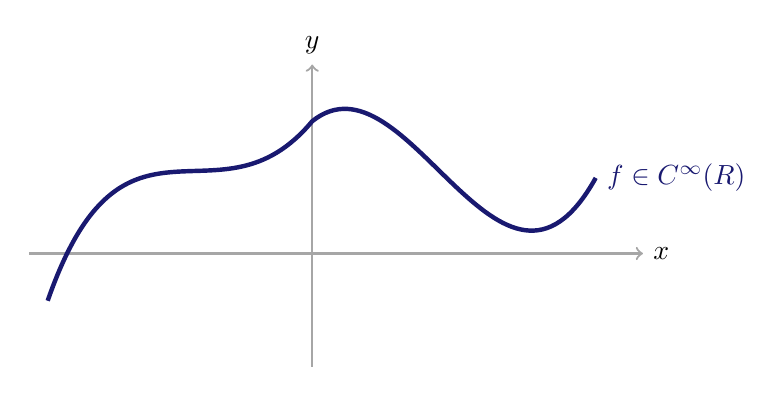
\begin{tikzpicture}[scale=1.2]
    \draw[->, thick, gray!70] (-3.0, 0) -- (3.5, 0) node[right, text=black] {$x$};
    \draw[->, thick, gray!70] (0, -1.2) -- (0, 2.0) node[above, text=black] {$y$};
    
    \draw[ultra thick, MidnightBlue] (-2.8, -0.5) 
        .. controls (-2.0, 1.8) and (-1.0, 0.2) .. (0.0, 1.4)
        .. controls (1.0, 2.2) and (2.0, -1.0) .. (3.0, 0.8)
        node[right] {$f \in C^\infty(\mathbb{R})$};
\end{tikzpicture}
\end{center}
\end{content}

\begin{speech}[01:00:50 - 01:02:05]
\inlinemetanote{A student asks a question about the board text}
Here? Which board? Infinitely differentiable function. 

Yeah, my handwriting's not good: function. And it's not because I have this wrist injury \inlinemetanote{laughs}; I just have bad handwriting. 

And I don't even know how I got this wrist injury. It's not like I'm an MMA fighter or anything like that. It just started hurting at one point. I thought it was going to be a career-ending injury, but it turns out that if I wear this thing, it's fine.
\end{speech}

\begin{speech}[01:02:05 - 01:03:45]
In this class, it's not primarily about such rings of differentiable functions --- that's some other class ---, but I can show you something interesting in it. 

There's an interesting ideal inside $C^\infty(\mathbb{R})$, and these are functions with compact support: $C_c^\infty(\mathbb{R})$. 

It's the set of functions with compact support. 

A general function can do whatever it wants, totally unconstrained. But a function with compact support means that its entire life happens somewhere compact. So it has to be zero here, and then suddenly it comes to life, and then it goes to zero. So it's like this kind of hat function that looks like that, okay? That's a function of compact support.
\end{speech}

\begin{speech}[01:03:45 - 01:05:10]
So, is this an ideal? 

To be an ideal, it has to be the case that zero's there, and very fortunately zero has compact support. What does not have compact support is the constant one function; that does not have compact support. 

So, this whatever it is, it's surely not a subring, because it does not have the constant one function. 

If you add compact support things, they have compact support, that's true. And the interesting thing is if I take a function of compact support and I multiply it by any function, it still has compact support, because once this function is zero, it just cannot be brought back to life, no matter how much you multiply. 

So, this is an example.
\end{speech}

\begin{content}[Compactly Supported Smooth Functions as an Ideal]
\begin{definition}[Functions with Compact Support]\label[definition]{def:compactly-supported-functions}
The set of smooth functions with \newterm{compact support} on $\mathbb{R}$, denoted $C_c^\infty(\mathbb{R})$, is:
\begin{equation}\label{eq:cc-infty-def}
C_c^\infty(\mathbb{R}) := \bigl\{ f \in C^\infty(\mathbb{R}) \;\big|\; \operatorname{supp}(f) \text{ is compact} \bigr\},
\end{equation}
where $\operatorname{supp}(f) := \overline{\{x \in \mathbb{R} \mid f(x) \neq 0\}}$ is bounded (i.e., $f(x) = 0$ outside some finite interval $[-M, M]$).
\end{definition}

\begin{center}
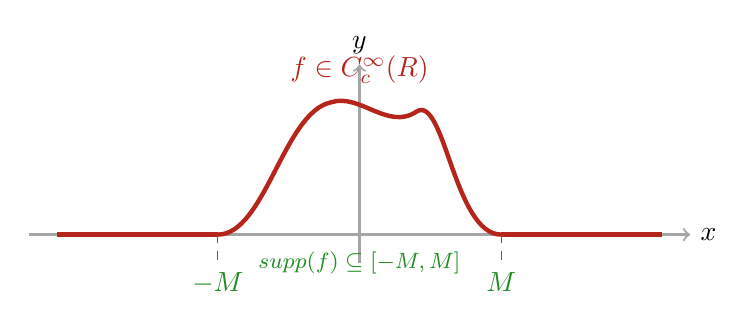
\begin{tikzpicture}[scale=1.2]
    \draw[->, thick, gray!70] (-3.5, 0) -- (3.5, 0) node[right, text=black] {$x$};
    \draw[->, thick, gray!70] (0, -0.3) -- (0, 1.8) node[above, text=black] {$y$};
    
    % Flat tails
    \draw[ultra thick, BrickRed] (-3.2, 0) -- (-1.5, 0);
    \draw[ultra thick, BrickRed] (1.5, 0) -- (3.2, 0);
    
    % Smooth bump (hat function)
    \draw[ultra thick, BrickRed] (-1.5, 0) 
        .. controls (-1.0, 0.0) and (-0.8, 1.3) .. (-0.3, 1.4)
        .. controls (0.0, 1.5) and (0.3, 1.1) .. (0.6, 1.3)
        .. controls (0.9, 1.5) and (1.0, 0.0) .. (1.5, 0);
        
    \node[BrickRed, above] at (0, 1.5) {$f \in C_c^\infty(\mathbb{R})$};
    \draw[dashed, ForestGreen] (-1.5, 0) -- (-1.5, -0.3) node[below] {$-M$};
    \draw[dashed, ForestGreen] (1.5, 0) -- (1.5, -0.3) node[below] {$M$};
    \node[ForestGreen, font=\footnotesize] at (0, -0.3) {$\operatorname{supp}(f) \subseteq [-M, M]$};
\end{tikzpicture}
\end{center}

\begin{proposition}\label[proposition]{prop:cc-infty-is-ideal}
$C_c^\infty(\mathbb{R})$ is an ideal of $C^\infty(\mathbb{R})$, but it is not a subring.
\end{proposition}

\begin{proof}
\begin{enumerate}[label=\textbf{(\arabic*)}]
    \item \textbf{Additive Subgroup:} The zero function $0 \in C_c^\infty(\mathbb{R})$ has $\operatorname{supp}(0) = \emptyset$. For $f, g \in C_c^\infty(\mathbb{R})$, $\operatorname{supp}(f + g) \subseteq \operatorname{supp}(f) \cup \operatorname{supp}(g)$, which is compact as the union of two compact sets.
    \item \textbf{Multiplicative Absorption (Ideal Property):} For any arbitrary $g \in C^\infty(\mathbb{R})$ and $f \in C_c^\infty(\mathbb{R})$,
    \[
    \operatorname{supp}(g \cdot f) \subseteq \operatorname{supp}(f).
    \]
    Since $\operatorname{supp}(f)$ is compact and closed subsets of compact sets in $\mathbb{R}$ are compact, $g \cdot f \in C_c^\infty(\mathbb{R})$.
    \item \textbf{Not a Subring:} The constant unit function $1(x) \equiv 1$ has $\operatorname{supp}(1) = \mathbb{R}$, which is not compact. Since $1 \notin C_c^\infty(\mathbb{R})$, $C_c^\infty(\mathbb{R})$ is not a subring.
\end{enumerate}
\end{proof}
\end{content}

\begin{speech}[01:05:10 - 01:06:40]
Maybe I ask you a question: is there some ideal $J$ that's bigger? 

Can you find an ideal that's bigger than this, and not the whole ring, of course, because that's always an ideal that's bigger? 

The traditional vision is there's an algebra direction, an analysis direction, a geometry direction. But actually, it doesn't really make sense to separate them all. It's all just one way of looking at numbers. 

Can you think of a way to make this ideal bigger?
\end{speech}

\begin{speech}[01:06:40 - 01:07:55]
Well, we used the fact that it's zero on both sides here, but it's not necessary, right? Can't we just say functions that eventually go to zero on the right? Those are more. And it satisfies the same thing. 

So here you could say $J$ is functions that become zero for all sufficiently large $x$. 

Those are functions that look like: they do whatever they want, and then eventually they become zero. These functions are certainly inside there, but there are more of them. 

And these things are also an ideal, because if you multiply by something that's zero here, it's going to stay zero.
\end{speech}

\begin{content}[A Strictly Larger Ideal: Functions Vanishing at Positive Infinity]
\begin{example}[Functions Vanishing for Large $x$]\label[example]{ex:ideal-vanishing-at-infinity}
Consider the set of smooth functions that vanish identically for all sufficiently large positive $x$:
\begin{equation}\label{eq:j-ideal-def}
J := \bigl\{ f \in C^\infty(\mathbb{R}) \;\big|\; \exists M \in \mathbb{R} \text{ such that } f(x) = 0 \text{ for all } x \ge M \bigr\}.
\end{equation}
\begin{itemize}
    \item \textbf{Proper Inclusions:} $C_c^\infty(\mathbb{R}) \subsetneq J \subsetneq C^\infty(\mathbb{R})$.
    Any compactly supported function vanishes for large $x$, so $C_c^\infty(\mathbb{R}) \subseteq J$. However, a function that is non-zero on all of $(-\infty, 0)$ and vanishes on $[1, \infty)$ belongs to $J \setminus C_c^\infty(\mathbb{R})$. Furthermore, $1 \notin J$, so $J \neq C^\infty(\mathbb{R})$.
    \item \textbf{Ideal Verification:} If $f \in J$ vanishes on $[M, \infty)$ and $g \in C^\infty(\mathbb{R})$, then $(g \cdot f)(x) = g(x) \cdot 0 = 0$ for all $x \ge M$, so $g \cdot f \in J$. Thus, $J$ is an ideal.
\end{itemize}

\begin{center}
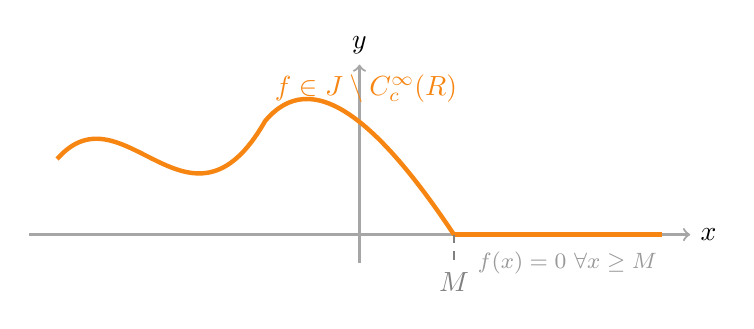
\begin{tikzpicture}[scale=1.2]
    \draw[->, thick, gray!70] (-3.5, 0) -- (3.5, 0) node[right, text=black] {$x$};
    \draw[->, thick, gray!70] (0, -0.3) -- (0, 1.8) node[above, text=black] {$y$};
    
    % Non-zero on left, decaying to 0 at M=1.0
    \draw[ultra thick, BurntOrange] (-3.2, 0.8) 
        .. controls (-2.5, 1.6) and (-1.8, -0.2) .. (-1.0, 1.2)
        .. controls (-0.5, 1.8) and (0.2, 1.2) .. (1.0, 0);
    \draw[ultra thick, BurntOrange] (1.0, 0) -- (3.2, 0);
    
    \draw[dashed, gray] (1.0, 0) -- (1.0, -0.3) node[below] {$M$};
    \node[BurntOrange, above right] at (-1.0, 1.3) {$f \in J \setminus C_c^\infty(\mathbb{R})$};
    \node[gray!80, font=\footnotesize] at (2.2, -0.3) {$f(x) = 0 \ \forall x \ge M$};
\end{tikzpicture}
\end{center}
\end{example}
\end{content}

\subsection{The Restriction Homomorphism}

\begin{speech}[01:07:55 - 01:09:12]
If I look at $C^\infty$ functions of $\mathbb{R}$, there's a ring homomorphism to $C^\infty$ functions of positive reals ($\mathbb{R}_{>0}$):
\[
C^\infty(\mathbb{R}) \xrightarrow{\operatorname{res}} C^\infty(\mathbb{R}_{>0}).
\]
This is a good example of a homomorphism. 

And this is called restriction, $\operatorname{res}$. 

Meaning if I have a $C^\infty$ function here, it's a function from all of $\mathbb{R}$ to $\mathbb{R}$. If I have one, I can just restrict it:
\[
f \colon \mathbb{R} \to \mathbb{R} \implies f|_{\mathbb{R}_{>0}} \colon \mathbb{R}_{>0} \to \mathbb{R}.
\]
Is that clear? Every element here, I can just restrict, and that gives me a map. First, it's a map on sets, and then you have to show it respects the zero, it respects the function that's constant $1$, and addition and multiplication behave well under restriction. So, this is a legitimate ring homomorphism. 

So for function spaces, restriction is a very useful way of making all these ring homomorphisms. 

Now your analysis question: is this surjective? 

That's properly a question in your analysis class. You can think about that.
\end{speech}

\begin{content}[The Restriction Homomorphism on Function Spaces]
\begin{definition}[Restriction Homomorphism]\label[definition]{def:restriction-homomorphism}
Let $U \subset \mathbb{R}$ be an open subset (e.g., $U = \mathbb{R}_{>0} = (0, \infty)$). The \newterm{restriction mapping}:
\begin{equation}\label{eq:restriction-map-def}
\operatorname{res} \colon C^\infty(\mathbb{R}) \to C^\infty(U), \quad f \mapsto f|_U
\end{equation}
is a ring homomorphism satisfying:
\begin{itemize}
    \item $\operatorname{res}(f + g) = (f + g)|_U = f|_U + g|_U = \operatorname{res}(f) + \operatorname{res}(g)$,
    \item $\operatorname{res}(f \cdot g) = (f \cdot g)|_U = f|_U \cdot g|_U = \operatorname{res}(f) \cdot \operatorname{res}(g)$,
    \item $\operatorname{res}(1_{\mathbb{R}}) = 1_U$.
\end{itemize}
\end{definition}
\end{content}

\section{Introduction to Category Theory}

\subsection{Categories, Objects, and Morphisms}

\begin{speech}[01:09:12 - 01:10:48]
There are two foundational topics which I've avoided discussing, but I think I'll discuss now. And it has to do with category theory and Zorn's lemma.

So, you had a foundations, this Grundstrukturen class. Did you discuss categories there?

You can say no.

Okay, so category. We discuss category. 

A category consists of objects and homs.

Homs are sometimes called morphisms, or arrows. The languages differ across different authors.

So, the first thing to know about a category: it has objects and it has homs.

More specifically, given two objects $A, B$ in the category, there is a set of homs, and this set has a name:
\[
\operatorname{Hom}(A, B).
\]
\end{speech}

\begin{content}[Foundational Data of a Category]
\begin{definition}[Category: Objects and Hom-Sets]\label[definition]{def:category-foundations}
A \newterm{category} $\mathcal{C}$ consists of:
\begin{enumerate}[label=\textbf{(\arabic*)}]
    \item A collection of \newterm{objects}, denoted $\operatorname{Obj}(\mathcal{C})$. We write $A \in \operatorname{Obj}(\mathcal{C})$ to indicate that $A$ is an object of $\mathcal{C}$.
    \item For every pair of objects $A, B \in \operatorname{Obj}(\mathcal{C})$, a set of \newterm{morphisms} (also called \newterm{homs} or \newterm{arrows}), denoted:
    \begin{equation}\label{eq:hom-set}
    \operatorname{Hom}_{\mathcal{C}}(A, B) \quad (\text{or } \operatorname{Mor}_{\mathcal{C}}(A, B)).
    \end{equation}
    An element $f \in \operatorname{Hom}_{\mathcal{C}}(A, B)$ is represented diagrammatically as an arrow $f \colon A \to B$ or $A \xrightarrow{f} B$, where $A$ is the \newterm{domain} (source) and $B$ is the \newterm{codomain} (target).
\end{enumerate}
\end{definition}
\end{content}

\subsection{Examples of Categories: Groups, Rings, and Vector Spaces}

\begin{speech}[01:10:48 - 01:12:06]
For example, the category of groups.

The category of groups has objects, and the objects are groups.

An object is a group $(G, \cdot, e)$. That's the objects. In the world of all groups, every possible group is in here. 

And what are the homs going to be? The homs between two particular groups are the set of group homomorphisms from $G$ to $\hat{G}$.

Another example is the category of rings. There the objects are rings with the full data, and the homs are ring homomorphisms.

From last year you could consider the category of vector spaces over the complex numbers: the objects are vector spaces over $\mathbb{C}$, and the homs are linear maps.

To be a category, I have to tell you what the objects are, given two objects I have to tell you what the homs are, and the resulting structure has to have some properties.
\end{speech}

\begin{speech}[01:12:06 - 01:13:00]
Did you figure out this question about the restriction homomorphism?

\inlinemetanote{A student in the lecture hall answers}
\end{speech}

\begin{student}[Student Answer]
I think $\sin(1/x)$...
\end{student}

\begin{speech}[01:13:00 - 01:14:00]
Yeah, so the answer is no, it's not surjective.

A picture is worth a thousand words. 

The picture is an element here that's not there: $\sin(1/x)$ oscillating near $x = 0$. \inlinemetanote{draws a sketch of $\sin(1/x)$ oscillating near $x = 0$ on the blackboard}

You should recognize that from your analysis class. You know this function, right?
\end{speech}

\begin{content}[Non-Surjectivity of Restriction and the Topologist's Sine Curve]
\begin{proposition}[Non-Surjectivity of Restriction]\label[proposition]{prop:restriction-not-surjective}
The restriction ring homomorphism:
\[
\operatorname{res} \colon C^\infty(\mathbb{R}) \to C^\infty(\mathbb{R}_{>0}), \quad f \mapsto f|_{\mathbb{R}_{>0}}
\]
is \textbf{not} surjective.
\end{proposition}

\begin{proof}
To show that $\operatorname{res}$ is not surjective, it suffices to exhibit a smooth function $g \in C^\infty(\mathbb{R}_{>0})$ that cannot be extended to any continuous (and hence no smooth) function $\tilde{g} \colon \mathbb{R} \to \mathbb{R}$.

Consider the oscillating function:
\begin{equation}\label{eq:sine-one-over-x}
g(x) := \sin\left(\frac{1}{x}\right) \quad \text{for } x > 0.
\end{equation}
Since the composition of smooth functions on $(0, \infty)$ is smooth, $g \in C^\infty(\mathbb{R}_{>0})$. However, as $x \to 0^+$, the argument $\frac{1}{x} \to \infty$, and $g(x)$ oscillates infinitely often between $-1$ and $+1$ on every neighborhood $(0, \varepsilon)$. Consequently, the limit $\lim_{x \to 0^+} \sin(1/x)$ does not exist. Thus, $g$ cannot be extended continuously to $x = 0$, proving that $g \notin \operatorname{Im}(\operatorname{res})$.
\end{proof}

\begin{center}
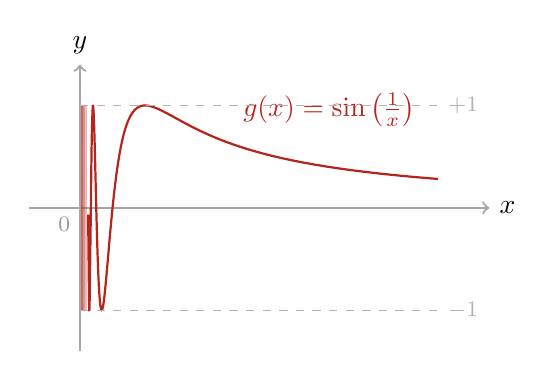
\begin{tikzpicture}[scale=1.3]
    \draw[->, thick, gray!70] (-0.5, 0) -- (4.0, 0) node[right, text=black] {$x$};
    \draw[->, thick, gray!70] (0, -1.4) -- (0, 1.4) node[above, text=black] {$y$};
    
    % Oscillating function sin(1/x)
    \draw[domain=0.08:3.5, samples=300, smooth, thick, BrickRed] 
        plot (\x, {sin((1.0 / \x) * 180 / 3.14159265)});
        
    % Dense oscillation region indicator near 0
    \draw[thick, BrickRed, opacity=0.7] (0.02, -1.0) -- (0.02, 1.0);
    \draw[thick, BrickRed, opacity=0.5] (0.04, -1.0) -- (0.04, 1.0);
    \draw[thick, BrickRed, opacity=0.3] (0.06, -1.0) -- (0.06, 1.0);
    
    \node[BrickRed, above right] at (1.5, 0.7) {$g(x) = \sin\left(\frac{1}{x}\right)$};
    \node[gray!80, font=\footnotesize, below left] at (0, 0) {$0$};
    \draw[dashed, gray!60] (0, 1) -- (3.5, 1) node[right, font=\footnotesize] {$+1$};
    \draw[dashed, gray!60] (0, -1) -- (3.5, -1) node[right, font=\footnotesize] {$-1$};
\end{tikzpicture}
\end{center}
\end{content}

\begin{content}[Standard Algebraic Categories]
\begin{example}[The Category of Groups $\mathbf{Grp}$]\label[example]{ex:cat-groups}
The \newterm{category of groups}, denoted $\mathbf{Grp}$, is defined by:
\begin{itemize}
    \item \textbf{Objects:} $\operatorname{Obj}(\mathbf{Grp}) = \bigl\{ (G, \cdot, e) \;\big|\; G \text{ is a group} \bigr\}$.
    \item \textbf{Morphisms:} For any two groups $G, \hat{G} \in \operatorname{Obj}(\mathbf{Grp})$,
    \begin{equation}\label{eq:grp-homs}
    \operatorname{Hom}_{\mathbf{Grp}}(G, \hat{G}) := \bigl\{ f \colon G \to \hat{G} \;\big|\; f \text{ is a group homomorphism} \bigr\}.
    \end{equation}
\end{itemize}
\end{example}

\begin{example}[The Category of Rings $\mathbf{Ring}$]\label[example]{ex:cat-rings}
The \newterm{category of rings}, denoted $\mathbf{Ring}$, is defined by:
\begin{itemize}
    \item \textbf{Objects:} $\operatorname{Obj}(\mathbf{Ring}) = \bigl\{ (R, +, \cdot, 0, 1) \;\big|\; R \text{ is a ring} \bigr\}$.
    \item \textbf{Morphisms:} For any two rings $R, \hat{R} \in \operatorname{Obj}(\mathbf{Ring})$,
    \begin{equation}\label{eq:ring-homs}
    \operatorname{Hom}_{\mathbf{Ring}}(R, \hat{R}) := \bigl\{ f \colon R \to \hat{R} \;\big|\; f \text{ is a ring homomorphism (with } f(1) = \hat{1}\text{)} \bigr\}.
    \end{equation}
\end{itemize}
\end{example}

\begin{example}[The Category of Vector Spaces $\mathbf{Vect}_{\mathbb{C}}$]\label[example]{ex:cat-vect}
The \newterm{category of complex vector spaces} $\mathbf{Vect}_{\mathbb{C}}$ is defined by:
\begin{itemize}
    \item \textbf{Objects:} Vector spaces $V$ over $\mathbb{C}$.
    \item \textbf{Morphisms:} Linear maps $T \colon V \to W$, so $\operatorname{Hom}_{\mathbf{Vect}_{\mathbb{C}}}(V, W) = \mathcal{L}(V, W)$.
\end{itemize}
\end{example}
\end{content}

\subsection{Axioms of a Category: Composition and Identity}

\begin{speech}[01:14:00 - 01:15:45]
Okay, so the properties that the homs have to satisfy for the category are very simple properties.

The first property is that $\operatorname{Hom}(A, B)$ is a set.

The second is that there's composition.

Composition means that if I have three objects, $A, B$, and $C$, then here I have the set of homs from $A$ to $B$, and homs from $B$ to $C$, and composition means there has to be a rule that tells you how, if you have a hom from $A$ to $B$ and a hom from $B$ to $C$, this gives me a hom from $A$ to $C$.

If I'm telling you a category, it's up to me to tell you how to compose homs. And in all examples, you just compose them as functions.

And inside $\operatorname{Hom}(A, A)$ there's a distinguished element, called the identity ($\operatorname{id}_A$). That's part of the data.
\end{speech}

\begin{speech}[01:15:45 - 01:17:26]
And there's one more condition, which is how the identity relates to composition. 

If you take the identity in $A$, and you take any element $f \in \operatorname{Hom}(A, B)$, then if I do the identity first and then I do $f$, what should this be equal to?

Yeah, $f$! That's the identity axiom:
\[
f \circ \operatorname{id}_A = f.
\]
And also the other way: if you do $f$ first and then $\operatorname{id}_B$, then this should just be $f$:
\[
\operatorname{id}_B \circ f = f.
\]

The data of this category is to capture what happens when we think about these algebraic objects abstractly. We have objects, we have homs, the homs compose, there's an identity hom, and they satisfy these identity properties and associativity.
\end{speech}

\begin{content}[The Axioms of a Category]
\begin{definition}[Category (Full Formal Definition)]\label[definition]{def:category-full}
A \newterm{category} $\mathcal{C}$ consists of the following data:
\begin{enumerate}[label=\textbf{(\arabic*)}]
    \item A collection $\operatorname{Obj}(\mathcal{C})$ of \newterm{objects}.
    \item For any two objects $A, B \in \operatorname{Obj}(\mathcal{C})$, a set $\operatorname{Hom}_{\mathcal{C}}(A, B)$ of \newterm{morphisms}.
    \item For any three objects $A, B, C \in \operatorname{Obj}(\mathcal{C})$, a \newterm{composition law}:
    \begin{equation}\label{eq:composition-law}
    \circ \colon \operatorname{Hom}_{\mathcal{C}}(B, C) \times \operatorname{Hom}_{\mathcal{C}}(A, B) \to \operatorname{Hom}_{\mathcal{C}}(A, C), \quad (g, f) \mapsto g \circ f.
    \end{equation}
    \item For every object $A \in \operatorname{Obj}(\mathcal{C})$, a distinguished \newterm{identity morphism}:
    \begin{equation}\label{eq:identity-morphism}
    \operatorname{id}_A \in \operatorname{Hom}_{\mathcal{C}}(A, A).
    \end{equation}
\end{enumerate}
These data are required to satisfy the following category axioms:
\begin{itemize}
    \item \textbf{Associativity of Composition:} For all $f \in \operatorname{Hom}_{\mathcal{C}}(A, B)$, $g \in \operatorname{Hom}_{\mathcal{C}}(B, C)$, and $h \in \operatorname{Hom}_{\mathcal{C}}(C, D)$,
    \begin{equation}\label{eq:category-associativity}
    (h \circ g) \circ f = h \circ (g \circ f).
    \end{equation}
    \item \textbf{Identity Axioms (Unit Laws):} For any morphism $f \in \operatorname{Hom}_{\mathcal{C}}(A, B)$, composing with the identity morphism from either the left or the right acts as the identity:
    \begin{equation}\label{eq:category-identity-laws}
    f \circ \operatorname{id}_A = f \quad \text{and} \quad \operatorname{id}_B \circ f = f.
    \end{equation}
\end{itemize}
\end{definition}

\begin{center}
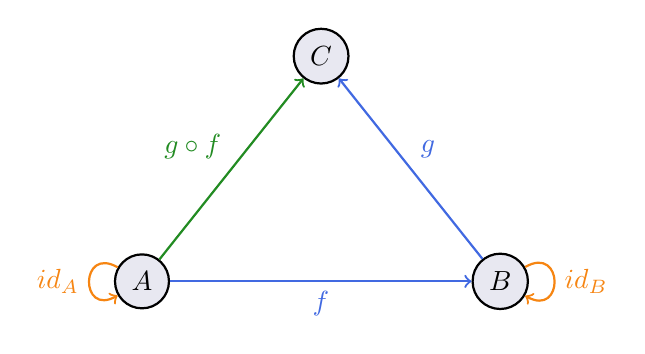
\begin{tikzpicture}[scale=1.3]
    \node (A) at (0,0) [circle, draw, fill=MidnightBlue!10, thick, font=\bfseries] {$A$};
    \node (B) at (3.5,0) [circle, draw, fill=MidnightBlue!10, thick, font=\bfseries] {$B$};
    \node (C) at (1.75,2.2) [circle, draw, fill=MidnightBlue!10, thick, font=\bfseries] {$C$};
    
    \draw[->, thick, RoyalBlue] (A) -- node[below] {$f$} (B);
    \draw[->, thick, RoyalBlue] (B) -- node[above right] {$g$} (C);
    \draw[->, thick, ForestGreen] (A) -- node[above left] {$g \circ f$} (C);
    
    % Identity loops
    \draw[->, thick, BurntOrange] (A) to[out=150, in=210, looseness=4] node[left] {$\operatorname{id}_A$} (A);
    \draw[->, thick, BurntOrange] (B) to[out=30, in=-30, looseness=4] node[right] {$\operatorname{id}_B$} (B);
\end{tikzpicture}
\end{center}
\end{content}

\subsection{Category-Theoretic Definition of Isomorphism}

\begin{speech}[01:17:26 - 01:19:58]
If you have a category, built into the category is a notion of isomorphic objects.

Suppose $\mathbf{Cat}$ is a category. I want to define the notion of isomorphism purely in categorical terms.

Is there a purely arrow-theoretic notion of isomorphism? Category-theoretic?

And the answer is yes.
\end{speech}

% [TIMESTAMP-SUSPECT: inspect manually — original: 01:19:58 - 01:22:08]
\begin{speech}[01:19:58 - 01:22:08]
So, I have this category $\mathbf{Cat}$, and I have two objects: $A$ and $B$. If I have $f \in \operatorname{Hom}(A, B)$, then $f$ is an isomorphism if...

What do you normally need for an isomorphism? You need a map the other way. 

If there exists a $g \in \operatorname{Hom}(B, A)$ going in the other direction such that what?
\end{speech}

\begin{student}[Student Answer]
The two compositions give the identity.
\end{student}

\begin{speech}[01:21:22 - 01:22:08]
Yeah, there exists a $g$ in the other direction such that:
\[
f \circ g = \operatorname{id}_B \quad \text{and} \quad g \circ f = \operatorname{id}_A.
\]
That's the definition. That's a purely category-theoretic definition of isomorphism.

Once I tell you the category of groups or rings, I tell you the homs, the identity, and this composition property, that already tells you what the notion of isomorphism is.
\end{speech}

\begin{content}[Categorical Isomorphisms]
\begin{definition}[Isomorphism in a Category]\label[definition]{def:categorical-isomorphism}
Let $\mathcal{C}$ be a category, and let $A, B \in \operatorname{Obj}(\mathcal{C})$. A morphism $f \in \operatorname{Hom}_{\mathcal{C}}(A, B)$ is called an \newterm{isomorphism} if there exists a morphism $g \in \operatorname{Hom}_{\mathcal{C}}(B, A)$ such that:
\begin{equation}\label{eq:categorical-isom-def}
g \circ f = \operatorname{id}_A \quad \text{and} \quad f \circ g = \operatorname{id}_B.
\end{equation}
The morphism $g$ is uniquely determined and is called the \newterm{inverse morphism} of $f$, denoted $g = f^{-1}$.

Two objects $A$ and $B$ are said to be \newterm{isomorphic} in $\mathcal{C}$ (written $A \cong B$) if there exists an isomorphism $f \in \operatorname{Hom}_{\mathcal{C}}(A, B)$.
\end{definition}

\begin{center}
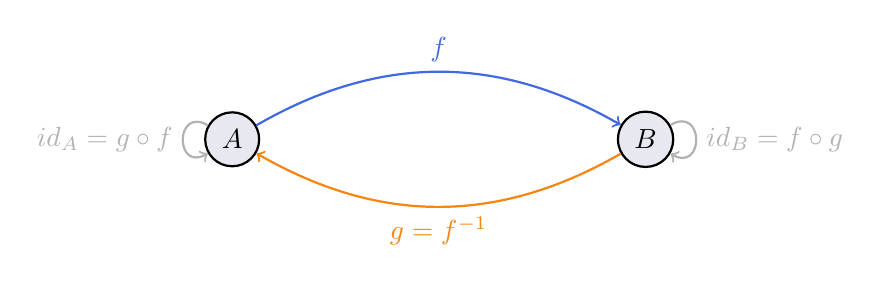
\begin{tikzpicture}[scale=1.5]
    \node (A) at (0,0) [circle, draw, fill=MidnightBlue!10, thick, font=\bfseries] {$A$};
    \node (B) at (3.5,0) [circle, draw, fill=MidnightBlue!10, thick, font=\bfseries] {$B$};
    
    \draw[->, thick, RoyalBlue] (A) to[bend left=30] node[above] {$f$} (B);
    \draw[->, thick, BurntOrange] (B) to[bend left=30] node[below] {$g = f^{-1}$} (A);
    
    \draw[->, thick, gray!60] (A) to[out=150, in=210, looseness=3.5] node[left] {$\operatorname{id}_A = g \circ f$} (A);
    \draw[->, thick, gray!60] (B) to[out=30, in=-30, looseness=3.5] node[right] {$\operatorname{id}_B = f \circ g$} (B);
\end{tikzpicture}
\end{center}

\begin{steps}[Arrow-Theoretic Universality of Isomorphisms]
Notice that \cref{def:categorical-isomorphism} makes \textbf{no reference to internal set elements, injectivity, or surjectivity}. Bijectivity is replaced purely by the existence of a two-sided structural inverse arrow. In concrete categories:
\begin{itemize}
    \item In $\mathbf{Grp}$, categorical isomorphisms are precisely bijective group homomorphisms.
    \item In $\mathbf{Ring}$, categorical isomorphisms are bijective ring homomorphisms.
    \item In $\mathbf{Vect}_K$, categorical isomorphisms are bijective linear transformations (invertible matrices).
\end{itemize}
\end{steps}
\end{content}

\begin{insight}[The Power of Category-Theoretic Abstraction]
Category theory unifies mathematics by defining concepts purely in terms of external interactions (\newterm{morphisms}) between systems rather than internal set elements. The definition of an isomorphism $g \circ f = \operatorname{id}_A$ and $f \circ g = \operatorname{id}_B$ is universally identical across group theory, ring theory, linear algebra, topology, and algebraic geometry.
\end{insight}

\section{Functors Between Categories}

\subsection{Definition of a Covariant Functor}

\begin{speech}[01:22:08 - 01:23:55]
There's a notion of functor.

A functor is a notion of a map from one category to another. Functors compare two different categories:
\[
F \colon \mathbf{Cat} \to \widehat{\mathbf{Cat}}.
\]

And now what's the data of the functor? 

For every object $A$ in the first category, I have to give you an object $F(A)$ in the second category. That's part of the data of the functor.
\end{speech}

\begin{speech}[01:23:55 - 01:25:28]
That's not enough: whenever I have an arrow $A \xrightarrow{f} B$ on the $\mathbf{Cat}$ side, I also have to tell you how this hom goes to a hom between these on the other side:
\[
F(f) \colon F(A) \to F(B).
\]

And it has to respect all of the structure, which means this rule must take the identity to the identities:
\[
F(\operatorname{id}_A) = \operatorname{id}_{F(A)},
\]
and it must respect composition:
\[
F(g \circ f) = F(g) \circ F(f).
\]
That's the notion of a functor.
\end{speech}

\begin{content}[Definition of a Covariant Functor]
\begin{definition}[Covariant Functor]\label[definition]{def:functor}
Let $\mathcal{C}$ and $\mathcal{D}$ be categories. A \newterm{(covariant) functor} $F \colon \mathcal{C} \to \mathcal{D}$ consists of:
\begin{enumerate}[label=\textbf{(\arabic*)}]
    \item An \textbf{Object Mapping}: Assigning to each object $A \in \operatorname{Obj}(\mathcal{C})$ an object $F(A) \in \operatorname{Obj}(\mathcal{D})$.
    \item A \textbf{Morphism Mapping}: Assigning to each morphism $f \in \operatorname{Hom}_{\mathcal{C}}(A, B)$ a morphism:
    \begin{equation}\label{eq:functor-morphism-map}
    F(f) \in \operatorname{Hom}_{\mathcal{D}}\bigl(F(A), F(B)\bigr).
    \end{equation}
\end{enumerate}
Such that the following two functoriality axioms are satisfied:
\begin{itemize}
    \item \textbf{Preservation of Identities:} For every object $A \in \operatorname{Obj}(\mathcal{C})$,
    \begin{equation}\label{eq:functor-identity}
    F(\operatorname{id}_A) = \operatorname{id}_{F(A)}.
    \end{equation}
    \item \textbf{Preservation of Composition:} For all composable morphisms $A \xrightarrow{f} B \xrightarrow{g} C$ in $\mathcal{C}$,
    \begin{equation}\label{eq:functor-composition}
    F(g \circ f) = F(g) \circ F(f).
    \end{equation}
\end{itemize}
\end{definition}

\begin{center}
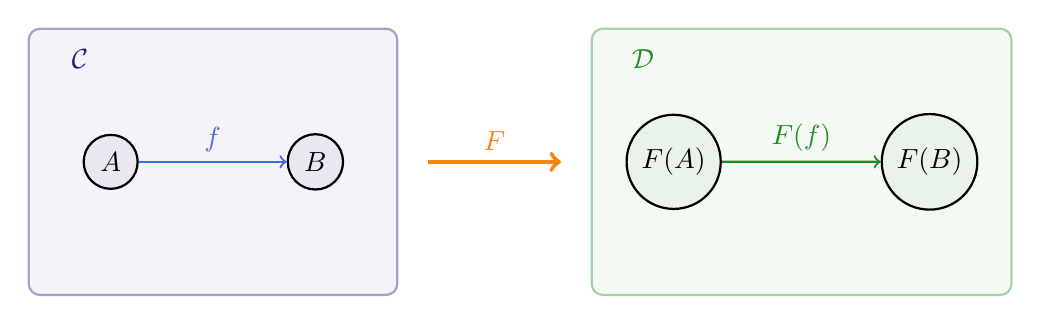
\begin{tikzpicture}[scale=1.3]
    % Category C Box
    \draw[thick, draw=MidnightBlue!40, fill=MidnightBlue!5, rounded corners] (-0.8,-0.8) rectangle (2.8,1.8);
    \node[MidnightBlue, font=\bfseries] at (-0.3, 1.5) {$\mathcal{C}$};
    \node (A) at (0,0.5) [circle, draw, fill=MidnightBlue!10, thick] {$A$};
    \node (B) at (2.0,0.5) [circle, draw, fill=MidnightBlue!10, thick] {$B$};
    \draw[->, thick, RoyalBlue] (A) -- node[above] {$f$} (B);
    
    % Category D Box
    \draw[thick, draw=ForestGreen!40, fill=ForestGreen!5, rounded corners] (4.7,-0.8) rectangle (8.8,1.8);
    \node[ForestGreen, font=\bfseries] at (5.2, 1.5) {$\mathcal{D}$};
    \node (FA) at (5.5,0.5) [circle, draw, fill=ForestGreen!10, thick] {$F(A)$};
    \node (FB) at (8.0,0.5) [circle, draw, fill=ForestGreen!10, thick] {$F(B)$};
    \draw[->, thick, ForestGreen] (FA) -- node[above] {$F(f)$} (FB);
    
    % Functor Arrow
    \draw[->, ultra thick, BurntOrange] (3.1, 0.5) -- node[above] {$F$} (4.4, 0.5);
\end{tikzpicture}
\end{center}
\end{content}

\subsection{Examples of Functors: The Forgetful Functor and the Double Dual Functor}

\begin{speech}[01:25:28 - 01:28:46]
What's an example of a functor? There's one that's been staring us in the face the whole time: if I take the category of rings, there's a way to get to the category of groups. It's just taking the additive structure of the ring. That's a rule to go from rings to groups, and that is a functor.

The first example of a functor is: take the category of rings $\mathbf{Ring}$ and the category of groups $\mathbf{Grp}$. There's a functor $F \colon \mathbf{Ring} \to \mathbf{Grp}$ defined by: if I take a ring $(R, +, \cdot, 0, 1)$, I associate to it the additive group $(R, +, 0)$.

And then if I have a ring homomorphism on the ring side, it also gives you an additive group homomorphism on the group side. That's the forgetful functor.
\end{speech}

\begin{content}[The Additive Forgetful Functor from Rings to Groups]
\begin{example}[The Additive Functor $\mathbf{Ring} \to \mathbf{Grp}$]\label[example]{ex:additive-forgetful-functor}
There is a canonical \newterm{forgetful functor} $F \colon \mathbf{Ring} \to \mathbf{Grp}$ mapping rings to their underlying additive abelian groups:
\begin{itemize}
    \item \textbf{On Objects:} For each ring $(R, +, \cdot, 0, 1) \in \operatorname{Obj}(\mathbf{Ring})$,
    \begin{equation}\label{eq:forgetful-obj}
    F\bigl((R, +, \cdot, 0, 1)\bigr) := (R, +, 0) \in \operatorname{Obj}(\mathbf{Grp}).
    \end{equation}
    \item \textbf{On Morphisms:} For any ring homomorphism $f \colon R \to \hat{R}$,
    \begin{equation}\label{eq:forgetful-mor}
    F(f) := f \colon (R, +, 0) \to (\hat{R}, +, \hat{0}).
    \end{equation}
    Since a ring homomorphism satisfies $f(a + b) = f(a) + f(b)$ and $f(0) = \hat{0}$, $F(f)$ is automatically a group homomorphism.
    \item \textbf{Functoriality:} $F(\operatorname{id}_R) = \operatorname{id}_{(R, +)}$ and $F(g \circ f) = g \circ f = F(g) \circ F(f)$ hold trivially.
\end{itemize}
\end{example}
\end{content}

\begin{speech}[01:28:46 - 01:30:08]
A more interesting example that you learned: if I take the category of complex vector spaces $\mathbf{Vect}_{\mathbb{C}}$, there's a very nice functor here to itself. 

This functor takes $V$ to its double dual $(V^*)^*$. 

If you take the dual $V^*$, it reverses the arrows (contravariant). But the double dual $(V^*)^*$ doesn't switch the arrows; it goes forward (covariant). Every vector space, you can associate its double dual.

And if you have a linear map $V \xrightarrow{T} W$, then the dual gives $W^* \xrightarrow{T^*} V^*$, and doing it again gives $(V^*)^* \xrightarrow{(T^*)^*} (W^*)^*$. 

So this functor associates $T \mapsto (T^*)^*$.
\end{speech}

% [TIMESTAMP-SUSPECT: inspect manually — original: 01:30:08 - 01:30:33]
\begin{speech}[01:30:08 - 01:30:33]
\inlinemetanote{A student asks a question about vector space dimensions}
\end{speech}

\begin{student}[Student Question]
Is the dimension of vector space only finite or can it also be infinite?
\end{student}

\begin{speech}[01:30:08 - 01:30:33]
I didn't say anything. You could, if you want, say you want the category of finite-dimensional vector spaces. But the way I said it, it is anything.

For finite-dimensional vector spaces it happens the double dual is isomorphic. I'm just saying there's a functor giving a vector space its double dual.

Usually in linear algebra you spend all your time dualing and double dualing, right? 

Okay, good. That's it. \inlinemetanote{students applaud / lecturer concludes the lecture}
\end{speech}

\begin{content}[The Double Dual Endofunctor on Vector Spaces]
\begin{example}[The Double Dual Functor on $\mathbf{Vect}_{\mathbb{C}}$]\label[example]{ex:double-dual-functor}
Let $\mathbf{Vect}_{\mathbb{C}}$ be the category of complex vector spaces and $\mathbb{C}$-linear maps. The \newterm{double dual operation} defines an \newterm{endofunctor} (a functor from a category to itself):
\[
(-)^{**} \colon \mathbf{Vect}_{\mathbb{C}} \to \mathbf{Vect}_{\mathbb{C}}
\]
defined by:
\begin{enumerate}[label=\textbf{(\arabic*)}]
    \item \textbf{On Objects:} For each vector space $V$,
    \begin{equation}\label{eq:double-dual-obj}
    V \mapsto V^{**} := (V^*)^* = \operatorname{Hom}_{\mathbb{C}}(V^*, \mathbb{C}).
    \end{equation}
    \item \textbf{On Morphisms:} For any linear map $T \colon V \to W$, the single dual map $T^* \colon W^* \to V^*$ reverses arrows (acting \newterm{contravariantly}: $T^*(\psi) = \psi \circ T$). Taking the dual a second time restores the original arrow direction, yielding the \newterm{double dual map}:
    \begin{equation}\label{eq:double-dual-mor}
    T^{**} := (T^*)^* \colon V^{**} \to W^{**}, \quad T^{**}(\xi) := \xi \circ T^*.
    \end{equation}
\end{enumerate}
\end{example}

\begin{center}
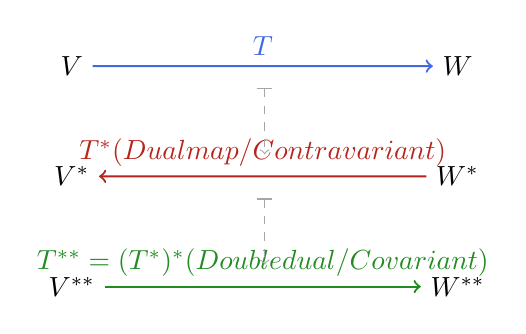
\begin{tikzpicture}[scale=1.4]
    \node (V) at (0, 2.0) [font=\bfseries] {$V$};
    \node (W) at (3.5, 2.0) [font=\bfseries] {$W$};
    \draw[->, thick, RoyalBlue] (V) -- node[above] {$T$} (W);
    
    \node (Wstar) at (3.5, 1.0) [font=\bfseries] {$W^*$};
    \node (Vstar) at (0, 1.0) [font=\bfseries] {$V^*$};
    \draw[->, thick, BrickRed] (Wstar) -- node[above] {$T^* \text{ (Dual map / Contravariant)}$} (Vstar);
    
    \node (Vstarstar) at (0, 0) [font=\bfseries] {$V^{**}$};
    \node (Wstarstar) at (3.5, 0) [font=\bfseries] {$W^{**}$};
    \draw[->, thick, ForestGreen] (Vstarstar) -- node[above] {$T^{**} = (T^*)^* \text{ (Double dual / Covariant)}$} (Wstarstar);
    
    \draw[|->, dashed, gray!70] (1.75, 1.8) -- (1.75, 1.2);
    \draw[|->, dashed, gray!70] (1.75, 0.8) -- (1.75, 0.2);
\end{tikzpicture}
\end{center}

\begin{steps}[Functoriality of Double Duality]
The composition of two arrow-reversing (contravariant) operations produces an arrow-preserving (covariant) functor:
\begin{itemize}
    \item \textbf{Preservation of Identities:} $(\operatorname{id}_V)^{**} = (\operatorname{id}_{V^*})^* = \operatorname{id}_{V^{**}}$.
    \item \textbf{Preservation of Composition:} For $U \xrightarrow{S} V \xrightarrow{T} W$, the dual satisfies $(T \circ S)^* = S^* \circ T^*$. Taking the dual again yields:
    \[
    (T \circ S)^{**} = (S^* \circ T^*)^* = (T^*)^* \circ (S^*)^* = T^{**} \circ S^{**}.
    \]
\end{itemize}
This holds for all vector spaces regardless of dimension. When $\dim(V) < \infty$, the canonical evaluation map $\operatorname{ev} \colon V \to V^{**}$, $v \mapsto (\psi \mapsto \psi(v))$ is an isomorphism, making $V \cong V^{**}$ a natural isomorphism of functors.
\end{steps}
\end{content}

\begin{overview}[Summary of Key Concepts]
This lecture established foundational concepts across modern abstract algebra and category theory:
\begin{itemize}
    \item \textbf{Groups, Rings, and Fields:} Reviewed core definitions, proving the uniqueness of identity elements and inverses. Explored the exponential isomorphism $(\mathbb{R}, +) \cong (\mathbb{R}_{>0}^*, \cdot)$ and proved $(\mathbb{R}^*, \cdot) \not\cong (\mathbb{R}_{>0}^*, \cdot)$ via torsion invariants.
    \item \textbf{Structure-Preserving Maps:} Formalized group and ring homomorphisms/isomorphisms. Analyzed how symmetry breaks between rings and groups: for group homomorphisms, kernels and images are subgroups; for ring homomorphisms, the kernel is an \emph{ideal} while the image is a \emph{subring}.
    \item \textbf{Substructures and Ideals:} Investigated subrings and ideals of $\mathbb{Z}$ (proving that $\mathbb{Z}$ is a Principal Ideal Domain where every ideal is $n\mathbb{Z}$) and smooth function rings $C^\infty(\mathbb{R})$ (where compactly supported functions $C_c^\infty(\mathbb{R})$ form an ideal).
    \item \textbf{Category Theory:} Introduced categories $\mathcal{C}$ (objects, hom-sets, composition, identity laws) and arrows-only definitions of categorical isomorphisms. Defined covariant functors $F \colon \mathcal{C} \to \mathcal{D}$ with canonical examples: the additive forgetful functor $\mathbf{Ring} \to \mathbf{Grp}$ and the double dual endofunctor $(-)^{**} \colon \mathbf{Vect}_{\mathbb{C}} \to \mathbf{Vect}_{\mathbb{C}}$.
\end{itemize}
\end{overview}